% =====================================================================
%  DESARROLLO POR OBJETIVOS (propuesta del 9 de noviembre)
%  Una sección por objetivo específico, con títulos tomados de lo que nombra cada objetivo.
%  Sin números de semana: el orden semana a semana está en el sitio del proyecto (anexo B).
%  Cada campaña y video se cita con el anexo A en su primera mención.
% =====================================================================
\chapter{Desarrollo}
\label{cap:desarrollo}

Cada objetivo específico se cumplió con actividades de las fases que fijó la metodología del anteproyecto: el levantamiento de requisitos y el diseño conceptual responden al primero; el desarrollo progresivo, al segundo y al tercero; la integración, a los tres; y la validación, al cuarto. El registro de cada semana, el código, la matriz de requisitos con la prueba de cada uno, el protocolo experimental y el registro de cada misión están en el repositorio y en el sitio del proyecto (anexo B).

% =====================================================================
\section{Primer objetivo específico: arquitectura funcional}
\label{sec:oe1}

Modelar la arquitectura funcional exigía definir los requerimientos, los escenarios de operación con múltiples pisos, la estrategia de asignación de tareas y el esquema de comunicación entre agentes.

\subsection{Requerimientos del sistema}

Los requerimientos se identificaron a partir de los objetivos específicos y del alcance del anteproyecto, que no los enumeraba, y se formalizaron en una matriz de treinta y seis requisitos, cada uno con su fuente y con la prueba que lo declara cumplido o no (tabla~\ref{tab:requisitos}). Veintinueve describen funciones del sistema y siete son restricciones del alcance, como operar en interiores y en condiciones controladas. Al primer objetivo le corresponden diez, sobre arquitectura, coordinación y relevo; al segundo, seis, sobre la plataforma; al tercero, seis, sobre la interfaz; y al cuarto, siete, sobre las métricas, el registro de cada misión y las dos campañas. La confirmación de cambio de piso y la cancelación no estaban en el anteproyecto y se añadieron al ver el sistema en uso.

Del alcance salieron las restricciones que condicionan el diseño: el edificio no se interviene y ningún agente cambia de piso. El punto de transferencia es, por lo tanto, la escalera, y el chasis puede conservar la dirección tipo automóvil, ya que ningún agente tiene que entrar a un ascensor ni subir escalones.

\begin{table}[H]
  \centering\footnotesize\setstretch{1.0}
  \caption{Matriz de los treinta y seis requisitos del sistema, por objetivo específico, con la prueba que verifica cada uno.}
  \label{tab:requisitos}
  \begin{tabular}{@{}c>{\raggedright\arraybackslash}p{0.42\textwidth}>{\raggedright\arraybackslash}p{0.47\textwidth}@{}}
    \toprule
    \textbf{N.\textsuperscript{o}} & \textbf{Requisito} & \textbf{Prueba que lo verifica} \\ \midrule
    \multicolumn{3}{@{}l}{\textit{Primer objetivo específico: arquitectura funcional}} \\
    1 & Dos agentes, uno por piso & Dos pilas de navegación, una por agente \\
    2 & Cada agente se direcciona por separado & Una orden a un agente no altera al otro \\
    3 & Órdenes solo con la acción de navegación & Nadie fuera de cada agente publica velocidades \\
    4 & Catálogo de puntos de interés con piso y pose & El coordinador publica el catálogo completo \\
    5 & Misión asignada al agente del piso de origen & La solicitud activa solo al agente de ese piso \\
    6 & Mismo piso: un agente y ningún relevo & Misión sin relevos, con el segundo agente libre \\
    7 & Pisos distintos: protocolo de relevo & Dos tramos y transferencia, con un relevo \\
    8 & Cada agente publica su estado a 2~Hz & Frecuencia medida y cambio de estado en la misión \\
    9 & Entorno de dos pisos con punto de transición & El mundo carga los dos pisos y se navega el superior \\
    10 & Comunicación entre agentes por el coordinador & Ningún agente se suscribe a tópicos del otro \\ \addlinespace
    \multicolumn{3}{@{}l}{\textit{Segundo objetivo específico: plataforma robótica}} \\
    11 & Locomoción con cinemática Ackermann & Recorrido medido contra la odometría \\
    12 & Láser utilizable para localización y evasión & Frecuencia nominal y obstáculos en el mapa de costos \\
    13 & Cada agente publica su odometría & Lectura antes y después de un desplazamiento conocido \\
    14 & Mando desde ROS~2, sin la interfaz del fabricante & Una orden desde otra máquina de la red mueve al agente \\
    15 & Red entre agentes con latencia acotada & Mediana $\leq$ 100~ms, percentil 95 $\leq$ 250~ms, sin pérdidas \\
    16 & Mismo código en simulación y en agentes físicos & Compila en las dos distribuciones y completa misiones \\ \addlinespace
    \multicolumn{3}{@{}l}{\textit{Tercer objetivo específico: interfaz móvil}} \\
    17 & Selección de origen y destino & La selección en listas del catálogo lanza una misión \\
    18 & Estado de la misión en texto legible & Texto del coordinador literal en cada etapa \\
    19 & La interfaz habla solo con el coordinador & El puente no expone ningún tópico de los agentes \\
    20 & Acceso desde el navegador de un teléfono & Carga y operación completa desde un teléfono \\
    21 & El segundo tramo espera la confirmación & Confirmar, confirmar tras el aviso y no confirmar \\
    22 & Cancelación y regreso a la escalera & Misión cancelada a mitad de tramo y una de control \\ \addlinespace
    \multicolumn{3}{@{}l}{\textit{Cuarto objetivo específico: evaluación experimental}} \\
    23 & Registro del tiempo de respuesta & La misión registra las marcas de los dos eventos \\
    24 & Registro del tiempo de asignación & Banco de pruebas con el reloj del sistema \\
    25 & Registro del éxito o fallo, con su motivo & Éxito y motivo quedan en el registro \\
    26 & Registro de la continuidad entre niveles & Ninguna etapa sin agente activo entre los dos tramos \\
    27 & Métricas obtenidas de un registro automático & Un archivo por misión, procesable sin intervención \\
    28 & Campaña en simulación con 30 repeticiones & Treinta registros válidos \\
    29 & Demostración física con 5 a 10 repeticiones & Registros de las misiones con los agentes físicos \\ \addlinespace
    \multicolumn{3}{@{}l}{\textit{Restricciones del alcance}} \\
    30 & Ningún agente cambia de piso & Altura de cada agente constante durante la misión \\
    31 & Sin manipular objetos ni intervenir el edificio & Por diseño: el agente solo tiene tracción y dirección \\
    32 & Interiores y condiciones controladas & En la campaña, sin personas ajenas a la prueba en el pasillo \\
    33 & Plataforma de bajo costo & AWS DeepRacer en lugar de DonkeyCar \\
    34 & Trayectorias aptas para dirección Ackermann & Radio mínimo y sin giro sobre el propio eje \\
    35 & Simulación a tiempo real & Factor de tiempo real de 0,99 o más \\
    36 & Operación en un entorno conocido y mapeado & El mapa es un insumo de la misión \\ \bottomrule
  \end{tabular}
\end{table}

\subsection{Escenarios de operación con múltiples pisos}
\label{sec:entornos}

Los escenarios se definieron en dos edificios de la sede principal de la Universidad Santo Tomás, Gregorio y Catalayud, con dos pisos en cada uno (tabla~\ref{tab:entornos}). Los pisos 2 y 3 del edificio Gregorio fueron el entorno de la simulación y de la primera prueba de navegación con un agente físico, y los pisos 3 y 4 del edificio Catalayud, el de las pruebas de verificación y la campaña con los agentes físicos.

\begin{table}[H]
  \centering\footnotesize\setstretch{1.0}
  \caption{Pisos en los que se probó el sistema, con su uso, su planta y sus puntos de interés.}
  \label{tab:entornos}
  \begin{tabular}{@{}>{\raggedright\arraybackslash}p{0.12\textwidth}>{\raggedright\arraybackslash}p{0.28\textwidth}>{\raggedright\arraybackslash}p{0.23\textwidth}>{\raggedright\arraybackslash}p{0.29\textwidth}@{}}
    \toprule
    \textbf{Piso} & \textbf{Uso} & \textbf{Planta} & \textbf{Puntos de interés} \\ \midrule
    Gregorio, piso 2 & Simulación; campaña de treinta misiones & Pasillo con un hall en un extremo; 41,0~m de extensión en su mapa & 15: doce salones ETM, almacén ETM, «Representación» y escalera \\ \addlinespace
    Gregorio, piso 3 & Simulación; campaña de treinta misiones; prueba de navegación con un agente físico & Pasillo con un hall al oeste; 46,9~m de extensión en su mapa & 16: dos laboratorios de sistemas, once aulas, sala de docentes, rama IEEE y escalera \\ \addlinespace
    Catalayud, piso 3 & Pruebas de verificación y campaña con los agentes físicos; comprobación en simulación & Pasillo de norte a sur, de 25,3 a 25,5~m de largo y de 2,35 a 2,45~m de ancho & 5: salones 301, 302 y 303, ascensor y escalera, a 22,1~m del extremo norte \\ \addlinespace
    Catalayud, piso 4 & Los mismos que el piso 3 & Pasillo de norte a sur, de 25,5 a 25,6~m de largo y de 2,35 a 2,61~m de ancho & 5: salones 401, 402 y 403, ascensor y escalera, a 24,4~m del extremo norte \\ \bottomrule
  \end{tabular}
\end{table}

Cada piso del edificio Gregorio es un mundo de Gazebo con su mapa de navegación y sus puntos de interés en el catálogo, y en los dos la escalera queda en un hall al extremo del pasillo (figura~\ref{fig:mapas-gregorio}). El anexo A, en su video 2, muestra al agente teleoperado en el modelo del piso 2 de ese edificio.

La prueba de navegación con un agente físico, en el hall del extremo oeste del piso 3 de Gregorio, no se superó: las dos llegadas medidas quedaron a 1,43 y 1,26~m del destino. El agente aún no tenía la unidad inercial, y la navegación no estaba ajustada para el agente físico, pues en esa misma sesión hubo que corregir una odometría invertida y subir el margen de llegada de Nav2 de 0,25 a 1,0~m. Además, el mapa cargado no correspondía al entorno real, dado que el mundo simulado del que salía daba el hall 0,84~m más ancho de lo que es, 4,24~m frente a 3,40~m, un 25~\% de error.

Con el mapa sin corregir, la localización terminó a 1,17~m de lado de la posición medida con flexómetro. Al corregirlo, ese error bajó a 0,15~m, aunque a lo largo del hall la separación llegó a 2,62~m, con la odometría del láser registrando el 73~\% del avance. La campaña en simulación no depende de esa diferencia, ya que en ella el mundo y el mapa salen del mismo modelo. Con los agentes físicos se cambió de edificio, dado que en Gregorio el tránsito de personas dificultaba las pruebas, el modelo no correspondía a la planta real y, en sus pasillos rectos y uniformes, la odometría del láser no registraba el avance.

\begin{figure}[H]
  \centering
  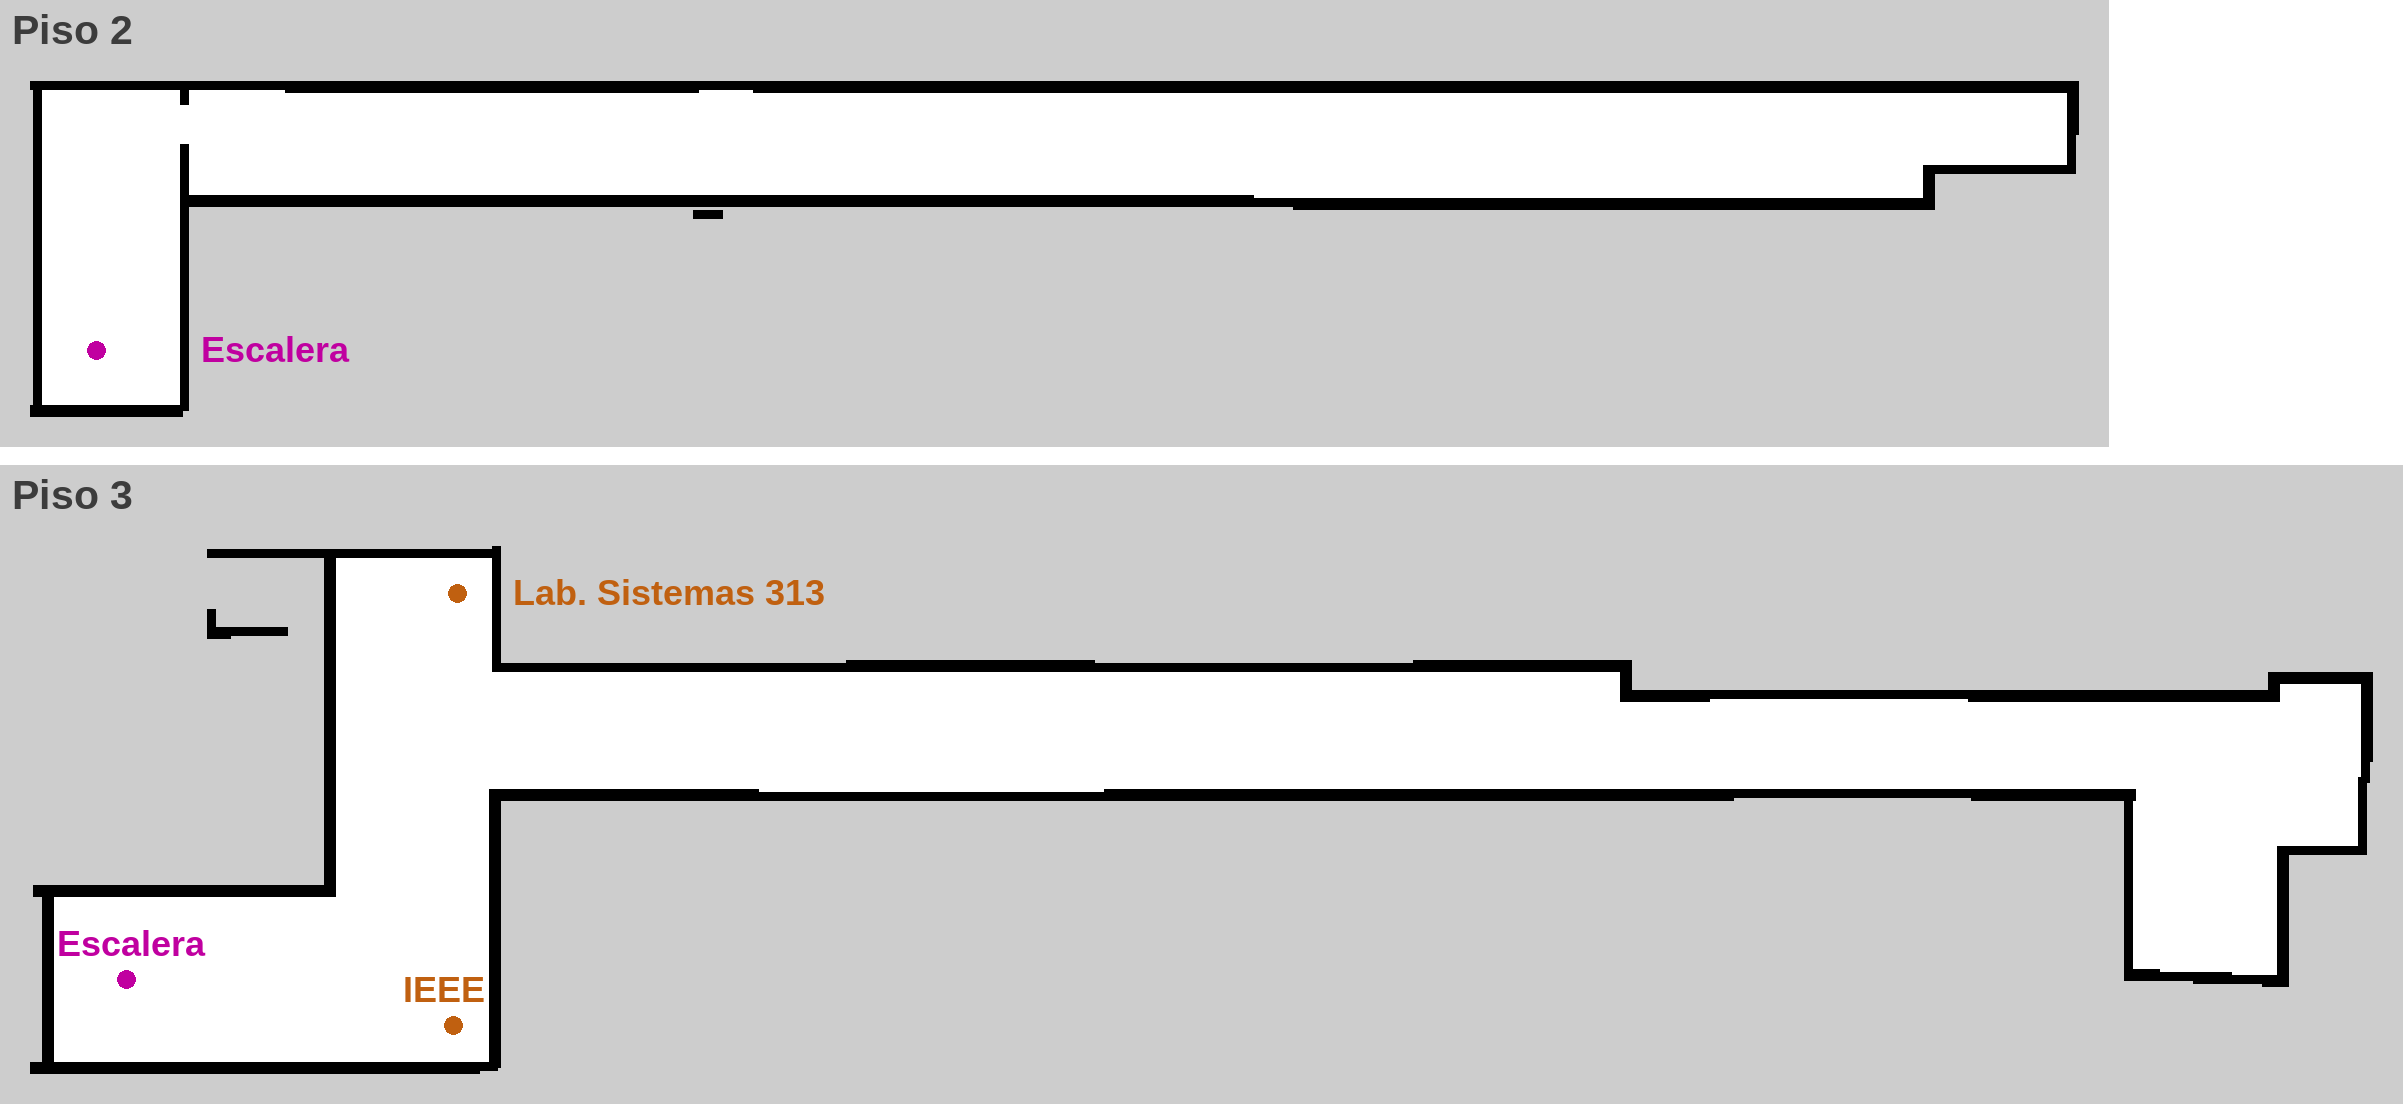
\includegraphics[width=0.72\textwidth]{imagenes/mapas_gregorio.png}
  \caption{Mapas de navegación de los pisos 2 (arriba) y 3 (abajo) del edificio Gregorio, calculados del modelo simulado, con el hall del piso 3 ya corregido.}
  \label{fig:mapas-gregorio}
\end{figure}

El edificio Catalayud se eligió con un criterio que salió de esa medida: como el agente estima su avance comparando barridos sucesivos del láser, necesita estructura no uniforme dentro del alcance del sensor durante todo el recorrido. Sus pisos 3 y 4 la tienen, ya que entre las hornacinas de los salones, los casilleros, la papelera, el ascensor y la escalera suman ocho cambios de perfil en 25~m, uno cada tres metros. Cada piso es un pasillo recto, con los tres salones al este, en hornacinas de 0,99 y 1,01~m de fondo, y el ascensor y la escalera al oeste (figura~\ref{fig:mapas-catalayud}).

\begin{figure}[H]
  \centering
  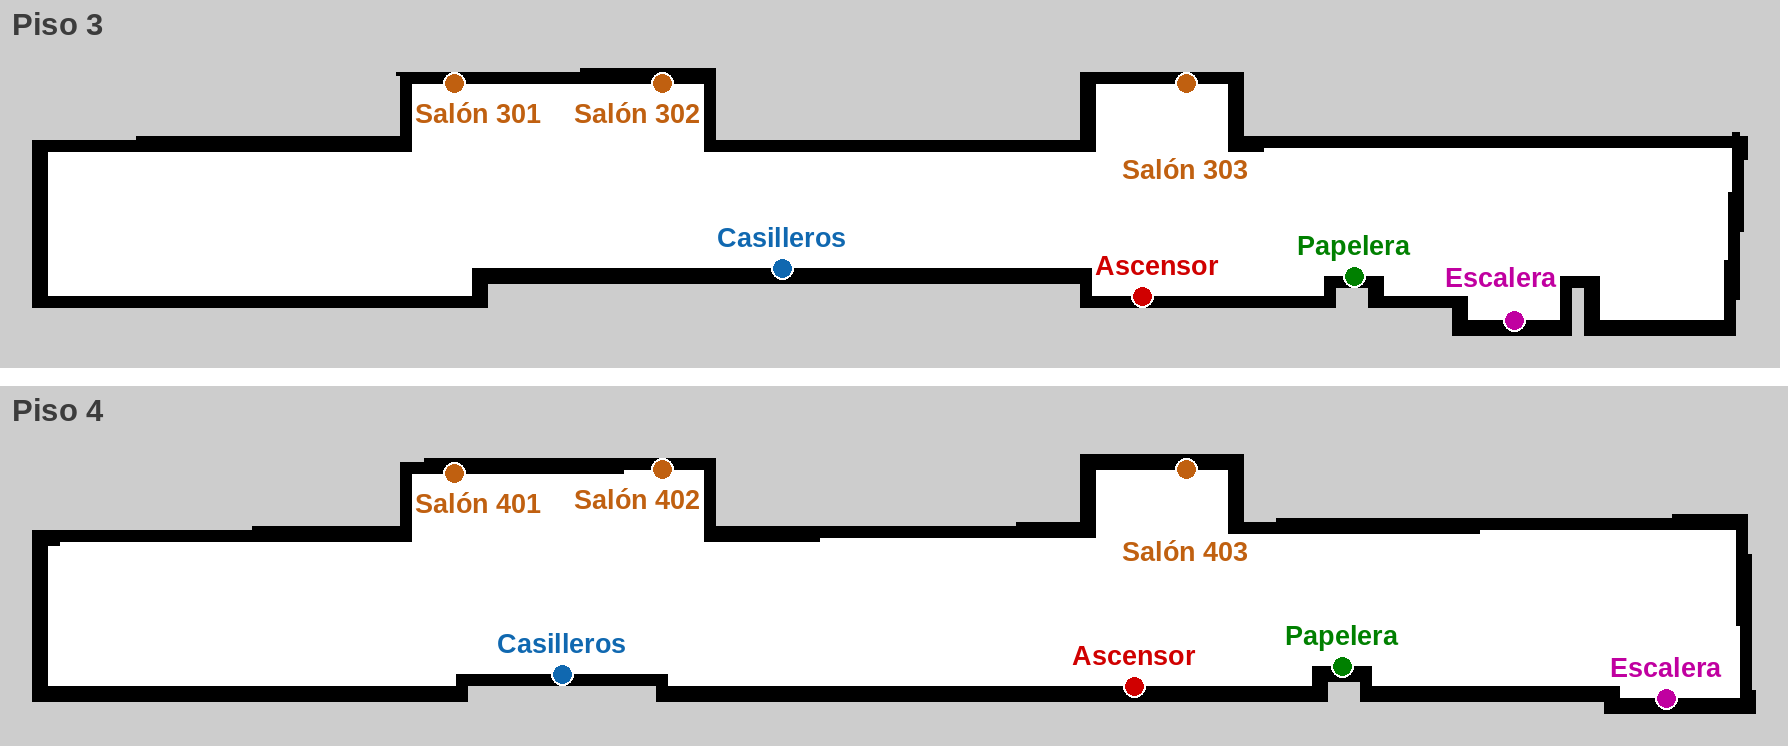
\includegraphics[width=0.76\textwidth]{imagenes/mapas_catalayud.png}
  \caption{Mapas de navegación de los pisos 3 (arriba) y 4 (abajo) del edificio Catalayud, derivados del levantamiento con flexómetro, con el extremo norte a la izquierda.}
  \label{fig:mapas-catalayud}
\end{figure}

El mapeo con SLAM en los propios agentes no entregó un mapa utilizable en ningún pasillo, por la misma falta de información de avance. Los pisos 3 y 4 del edificio Catalayud se levantaron entonces con flexómetro, y de ese levantamiento se derivaron el mundo simulado, el mapa de navegación y el catálogo de destinos, de manera que simulación y edificio coinciden al salir de la misma fuente. La herramienta que genera las plantas suma las dos paredes de cada pasillo y avisa si no cierran dentro del 2~\%; las plantas cierran al 0,62~\% en el piso 3 y al 0,32~\% en el piso 4.

\subsection{Arquitectura general y módulos}

La arquitectura consta de una interfaz web por la que entra la solicitud, un coordinador que la reparte y dos agentes, uno por piso, con su pila de navegación (figura~\ref{fig:arquitectura}). Ningún agente atraviesa la zona de transición: la cruza el usuario, y lo que se traspasa entre agentes en la escalera es la responsabilidad de guiarlo.

\begin{figure}[H]
  \centering
  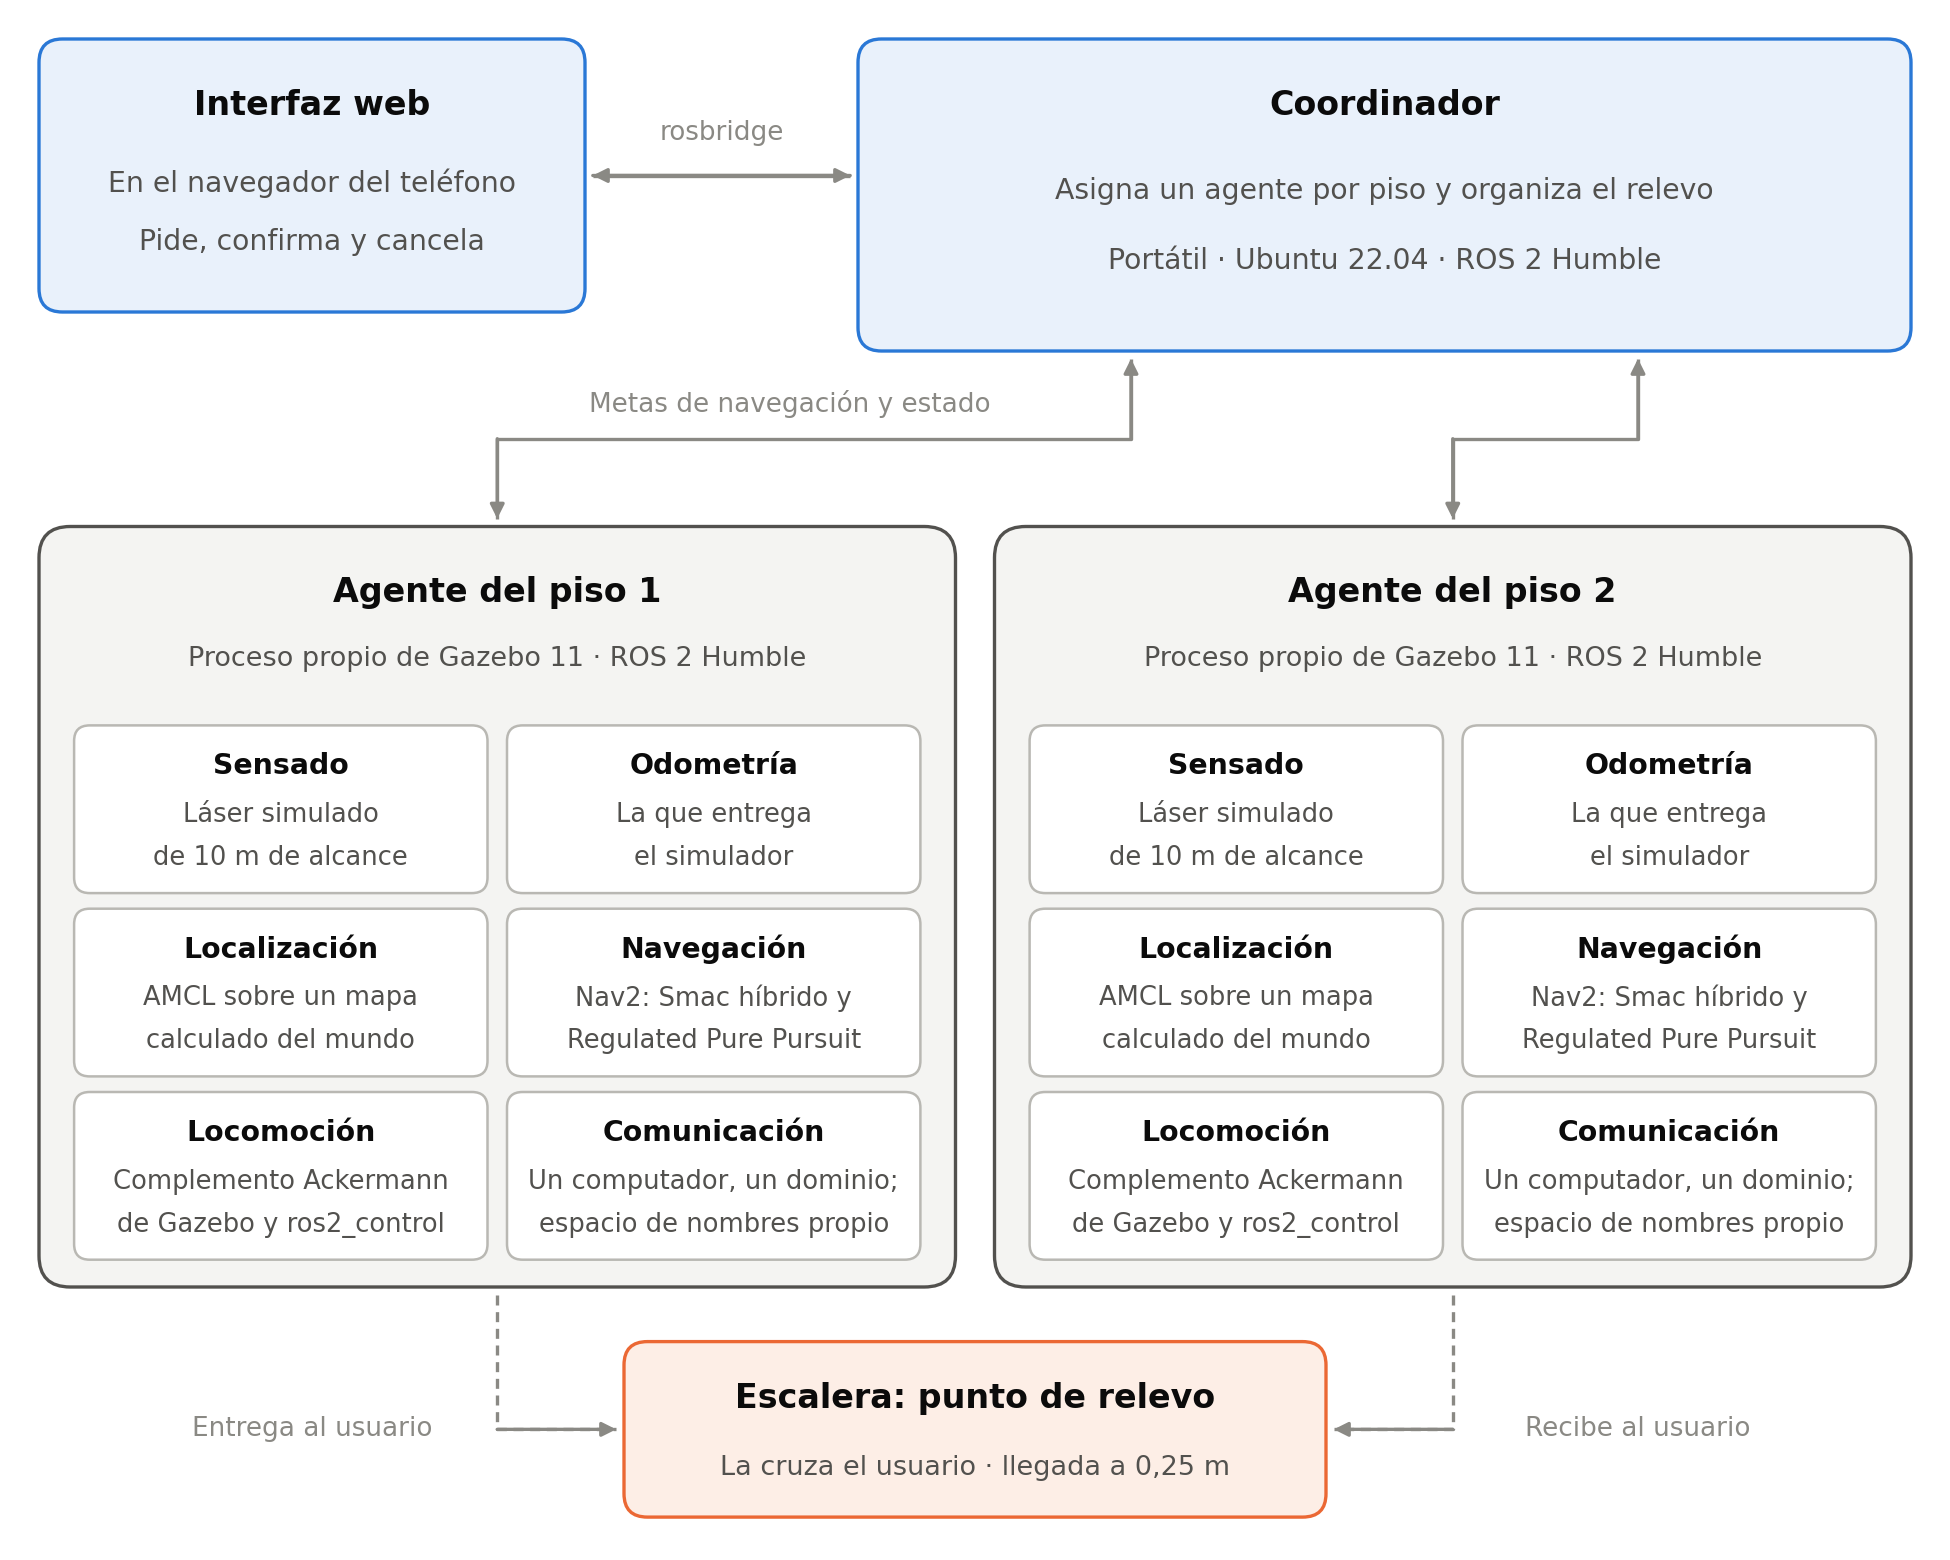
\includegraphics[width=0.9\textwidth]{imagenes/arquitectura_simulacion.png}
  \caption{Arquitectura del sistema en simulación.}
  \label{fig:arquitectura}
\end{figure}

Sus módulos son percepción, localización, planificación, control, locomoción, comunicación, coordinación e interfaz. Los cinco primeros se ejecutan en cada agente, la coordinación y la interfaz se sirven desde el portátil, y la comunicación los enlaza. La figura~\ref{fig:nodos} muestra los nodos principales en la campaña con los agentes físicos y lo que circula entre ellos, con los componentes del fabricante en borde discontinuo, y el anexo C enlaza el grafo completo, obtenido en simulación.

El funcionamiento se definió como un escenario de relevo en siete pasos. El usuario hace la solicitud, el coordinador asigna el agente y el agente del piso de origen recoge al usuario y lo guía hasta la escalera, donde lo entrega. El coordinador notifica entonces al agente del otro piso, que va a su punto de transferencia, el sistema espera a que el usuario confirme que cambió de piso y el guiado se reanuda en el piso de destino.

\begin{figure}[H]
  \centering
  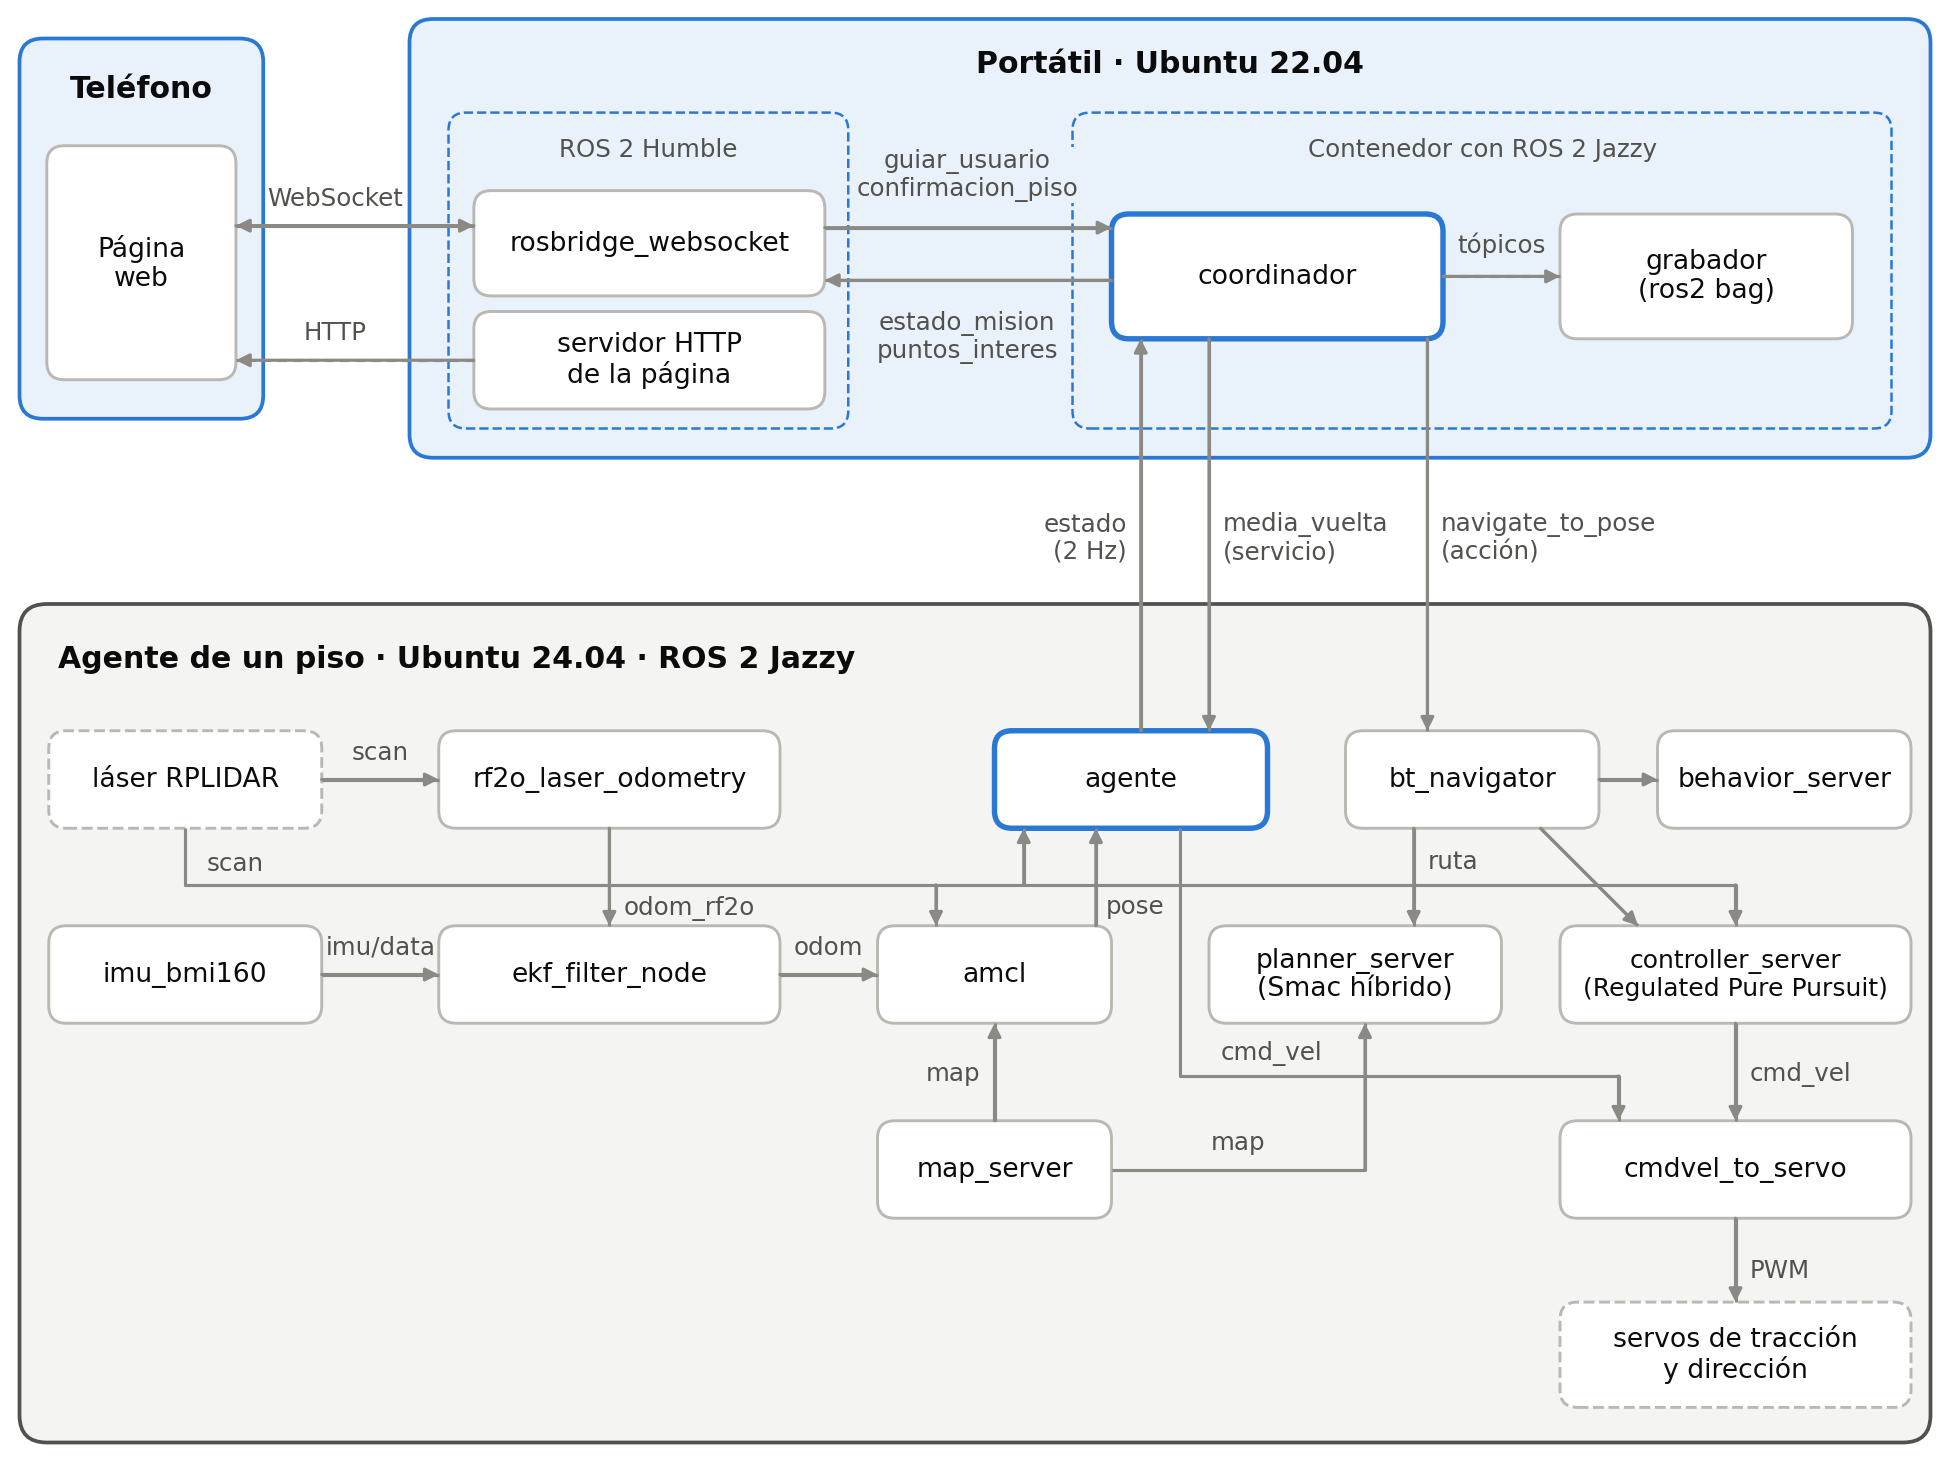
\includegraphics[width=\textwidth]{imagenes/nodos_sistema.png}
  \caption{Nodos principales de ROS~2 en la campaña con los agentes físicos.}
  \label{fig:nodos}
\end{figure}

\subsection{Estrategia de asignación de tareas}
\label{sec:planificador}
\label{sec:asignacion}

Cada piso tiene un agente asignado, esa correspondencia es un dato de configuración, y el coordinador elige el agente al aceptar la solicitud, según el piso del origen y del destino (anexo A, video 5). El relevo es el aporte declarado del proyecto, de modo que su planificación se escribió como una función pura, sin dependencia de ROS~2 ni estado propio (figura~\ref{fig:planificador}). Entran el catálogo de puntos y un par origen-destino, y salen los tramos que hay que ejecutar o un error con su motivo, antes de que ningún agente se mueva. Si el origen y el destino están en el mismo piso, la misión tiene dos tramos del mismo agente: ir a recoger al usuario y llevarlo al destino. Si están en pisos distintos, tiene cuatro: los dos anteriores, terminando en el punto de transferencia del piso de origen; el desplazamiento del segundo agente a su punto de transferencia; y el guiado final.

\begin{figure}[H]
  \centering
  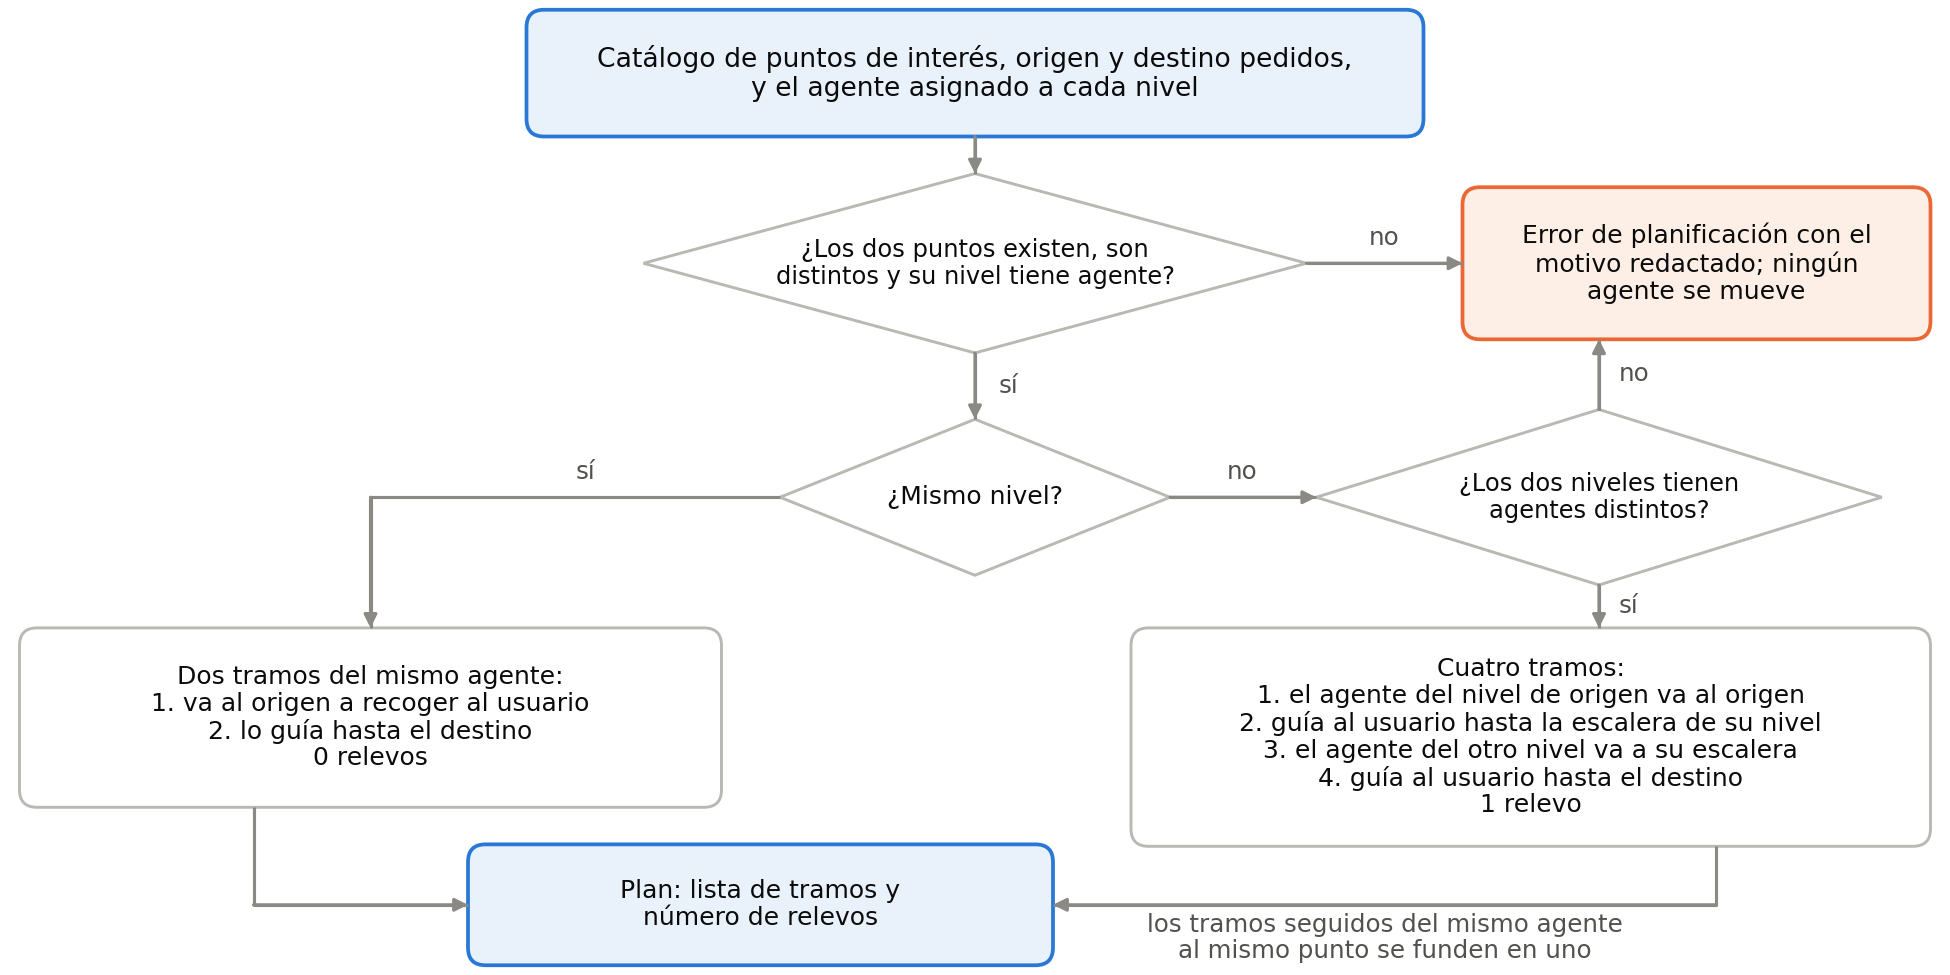
\includegraphics[width=0.93\textwidth]{imagenes/planificador.png}\hspace*{1.04cm}
  \caption{Función que planifica una misión.}
  \label{fig:planificador}
\end{figure}

Como función pura, una prueba automática la recorre entera en milisegundos y sin simulador. El catálogo de los pisos 2 y 3 del edificio Gregorio tiene 31 puntos de interés, y cada par ordenado de dos puntos distintos es una solicitud posible: $31 \times 30 = 930$ combinaciones. La prueba planifica las 930 y comprueba en todas que el plan empieza en el origen y termina en el destino, que ningún agente recibe una meta fuera de su piso y que una misión de dos pisos usa los dos agentes y un relevo. Con ella se encontró que, cuando el origen o el destino era el propio punto de transferencia de su piso, el plan mandaba al mismo agente dos veces a la misma pose, un defecto que quedó corregido. El planificador exige además un único punto de transferencia por piso.

\subsection{Esquema de comunicación entre agentes}
\label{sec:contrato}

El esquema se fijó en un contrato de interfaces que define qué habla con qué y en qué formato (tabla~\ref{tab:contrato}), implementado como un paquete propio de mensajes. La comunicación sigue tres reglas:
\begin{itemize}[leftmargin=*]
  \item el coordinador manda a un agente solo mediante la acción de navegación de ROS~2 o la petición de una media vuelta, sin publicar velocidades;
  \item la interfaz habla solo con el coordinador;
  \item el texto que ve el usuario lo redacta el coordinador, y la interfaz lo muestra literal, lo que evita tener dos copias de la misma lógica.
\end{itemize}
Cada cambio de etapa (tabla~\ref{tab:etapas-mision}) se publica, y esas publicaciones son las marcas de tiempo con que se calculan las métricas.

\begin{table}[H]
  \centering\footnotesize\setstretch{1.0}
  \caption{Interfaces del contrato entre la interfaz web, el coordinador y los agentes, donde \texttt{N} es el número del agente.}
  \label{tab:contrato}
  \begin{tabular}{@{}>{\scriptsize\raggedright\arraybackslash}p{0.285\textwidth}>{\raggedright\arraybackslash}p{0.12\textwidth}>{\raggedright\arraybackslash}p{0.195\textwidth}>{\raggedright\arraybackslash}p{0.32\textwidth}@{}}
    \toprule
    \footnotesize\textbf{Interfaz} & \textbf{Tipo} & \textbf{Sentido} & \textbf{Contenido} \\ \midrule
    \texttt{/coordinacion/guiar\_usuario} & acción propia & interfaz $\rightarrow$ coordinador & Origen y destino; estado durante la misión; éxito, tiempo, relevos o motivo del fallo \\
    \texttt{/coordinacion/estado\_mision} & tópico propio, 1~Hz & coordinador $\rightarrow$ interfaz & Etapa, agente activo, destino, distancia restante y texto para el usuario \\
    \texttt{/coordinacion/puntos\_interes} & tópico propio & coordinador $\rightarrow$ interfaz & Catálogo de puntos de interés, con su piso \\
    \texttt{/coordinacion/confirmacion\_piso} & tópico de texto & interfaz $\rightarrow$ coordinador & Confirmación del cambio de piso \\
    \texttt{/robotN/navigate\_to\_pose} & acción de Nav2 & coordinador $\rightarrow$ agente & Meta de cada tramo \\
    \texttt{/robotN/media\_vuelta} & servicio & coordinador $\rightarrow$ agente & Media vuelta antes de una meta que queda detrás \\
    \texttt{/robotN/estado} & tópico propio, 2~Hz & agente $\rightarrow$ coordinador & Piso, pose en el mapa y estado del agente \\
    \texttt{/robotN/odom} & odometría & agente $\rightarrow$ coordinador & Desplazamiento, para marcar el primer movimiento \\ \bottomrule
  \end{tabular}
\end{table}

\begin{table}[H]
  \centering\footnotesize\setstretch{1.0}
  \caption{Etapas de una misión, tal como las publica el coordinador.}
  \label{tab:etapas-mision}
  \begin{tabular}{@{}>{\raggedright\arraybackslash}p{0.27\textwidth}>{\raggedright\arraybackslash}p{0.65\textwidth}@{}}
    \toprule
    \textbf{Etapa} & \textbf{Significado} \\ \midrule
    Recibida & El coordinador aceptó la solicitud y todavía no asignó agente \\
    Primer tramo & El agente del piso de origen va a recoger al usuario y lo guía \\
    Transferencia & El agente del otro piso va a su punto de transferencia \\
    Esperando confirmación & El sistema espera que el usuario confirme que ya cambió de piso \\
    Segundo tramo & El agente del piso de destino guía al usuario hasta el final \\
    Completada & La misión terminó con la llegada verificada \\
    Fallida & La misión terminó sin cumplirse, con el motivo en el texto \\
    Cancelando & El usuario canceló y el agente activo regresa a su punto de transferencia \\
    Inactiva & No hay misión en curso \\ \bottomrule
  \end{tabular}
\end{table}

% =====================================================================
\section{Segundo objetivo específico: plataforma robótica}
\label{sec:plataforma}

El sistema se cargó en dos agentes de la plataforma AWS DeepRacer (figura~\ref{fig:agentes-fisicos}), cada uno a cargo de un piso del edificio Catalayud, y en ellos se integraron los módulos de locomoción, sensado, procesamiento y comunicación que nombra el objetivo. La tabla~\ref{tab:vehiculo} reúne los componentes del sistema.

\begin{figure}[H]
  \centering
  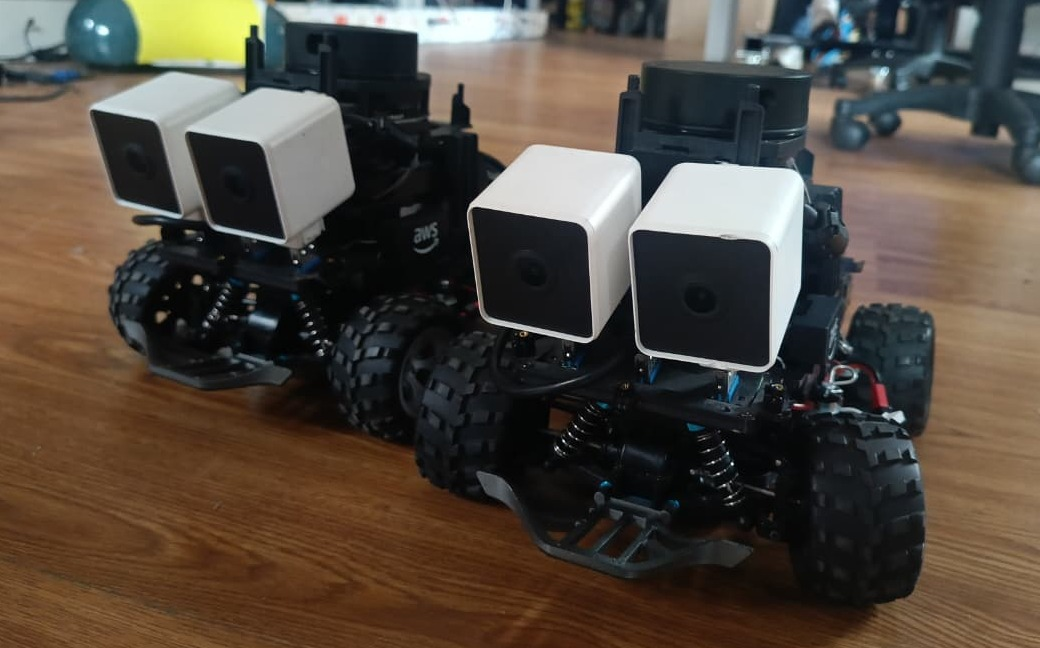
\includegraphics[width=0.5\textwidth]{imagenes/agentes_fisicos.jpg}
  \caption{Los dos agentes físicos, con el sistema cargado en la plataforma AWS DeepRacer.}
  \label{fig:agentes-fisicos}
\end{figure}

\begin{table}[H]
  \centering\footnotesize\setstretch{1.0}
  \caption{Lista de componentes del sistema.}
  \label{tab:vehiculo}
  \begin{tabular}{@{}>{\raggedright\arraybackslash}p{0.23\textwidth}c>{\raggedright\arraybackslash}p{0.62\textwidth}@{}}
    \toprule
    \textbf{Componente} & \textbf{Cant.} & \textbf{Descripción} \\ \midrule
    \multicolumn{3}{@{}l}{\textit{Agentes}} \\
    Chasis & 2 & AWS DeepRacer, escala 1:18, dirección Ackermann, motor de tracción con variador y servomotor de dirección \\
    Tarjeta de cómputo & 2 & Tarjeta original, procesador Intel Atom E3930 de dos núcleos, 4~GB de memoria; Ubuntu 24.04 y ROS~2 Jazzy \\
    Láser & 2 & RPLIDAR A1M8-R5, por USB: 360$^\circ$, 360 muestras por barrido, alcance de 0,15 a 12~m, entre 6,8 y 7~Hz \\
    Unidad inercial & 2 & Bosch BMI160 integrada en la tarjeta, por I2C: giroscopio y acelerómetro \\
    Cámaras & 2 pares & Estéreo; desactivadas por software: el sistema no las usa y cargaban la tarjeta \\
    Batería de cómputo & 2 & Alimenta la tarjeta \\
    Batería de tracción & 2 & Polímero de litio \\ \addlinespace
    \multicolumn{3}{@{}l}{\textit{Coordinación e interacción}} \\
    Portátil & 1 & Ubuntu 22.04 y ROS~2 Humble (AMD Ryzen 5 PRO 5650U, 16~GB); el coordinador se ejecuta en un contenedor con Jazzy \\
    Teléfono & 1 & Abre la interfaz web, conectado a la red de los agentes \\ \addlinespace
    \multicolumn{3}{@{}l}{\textit{Red}} \\
    Enrutador & 1 & TP-Link TL-WR940N: reparte las direcciones de la red y da un enlace de respaldo a 2,4~GHz \\
    Puntos de acceso & 2 & FiberHome, uno por piso del edificio Catalayud, en modo puente: 5~GHz, canal 44 en el piso 3 y 36 en el piso 4 \\
    Cables de red & 2 & Del enrutador a cada punto de acceso, entre puertos LAN: uno en el mismo piso y otro entre pisos \\ \addlinespace
    \multicolumn{3}{@{}l}{\textit{Medición}} \\
    Flexómetro & 1 & Levantamiento de las plantas y medida del avance y de la llegada en las pruebas de odometría y de navegación \\ \bottomrule
  \end{tabular}
\end{table}

\subsection{Selección de la plataforma y del simulador}
\label{sec:donkeycar}

El anteproyecto planteó construir los agentes sobre DonkeyCar, una plataforma abierta de vehículos a escala con dirección tipo automóvil \autocite{donkeycar}, con una Raspberry Pi~4, simulación en CoppeliaSim y visión con OpenCV. Para analizarla se instaló su simulador y se empezó un modelo propio del agente para ROS~2 (figura~\ref{fig:etapas-plataforma}, izquierda). Ese simulador no se comunica con ROS~2, de modo que no permite probar el mapeo, la localización ni la comunicación entre agentes, y no existía un modelo para Gazebo con dirección Ackermann que funcionara en ROS~2 Humble.

Para el simulador se fijaron cuatro criterios: compatibilidad con ROS~2 Humble, vehículos con dirección Ackermann, entornos interiores y soporte para mapeo y navegación. Entre CoppeliaSim, el simulador del curso F1TENTH y Gazebo \autocite{koenig2004gazebo}, se eligió Gazebo por su integración directa con ROS~2 y con su sistema de control de articulaciones.

Como plataforma se adoptó AWS DeepRacer. Es la misma clase de vehículo que el DonkeyCar, AWS publicó en código abierto su modelo de simulación con un complemento de cinemática Ackermann para Gazebo \autocite{awsdeepracer2021}, y el laboratorio de robótica de la universidad ya contaba con dos, con lo que el tiempo disponible pudo dedicarse a la coordinación. El costo fue convivir con el software del fabricante, cuyos nodos ocupan el láser, se ejecutan con el usuario administrador y publican sin espacio de nombres. La tarjeta original, además, solo admite el software de la comunidad \autocite{deepracercustomcar} sobre Ubuntu 24.04 y ROS~2 Jazzy, y la integración de Gazebo~11 con ROS~2 no está publicada para Jazzy, de manera que el proyecto trabaja con dos distribuciones.

\begin{figure}[H]
  \centering
  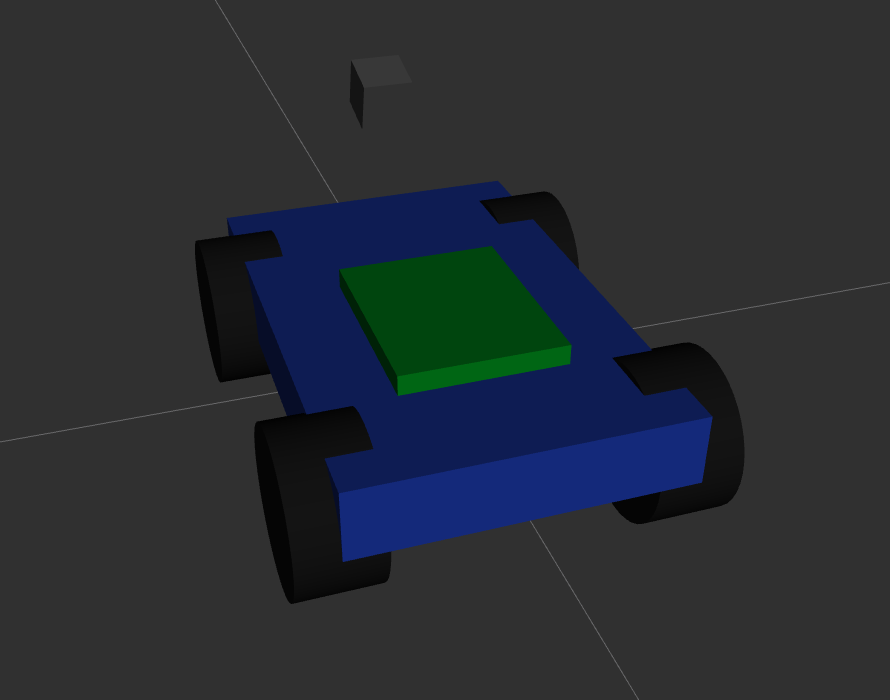
\includegraphics[height=3.2cm]{imagenes/etapa_donkeycar_modelo.png}\hfill
  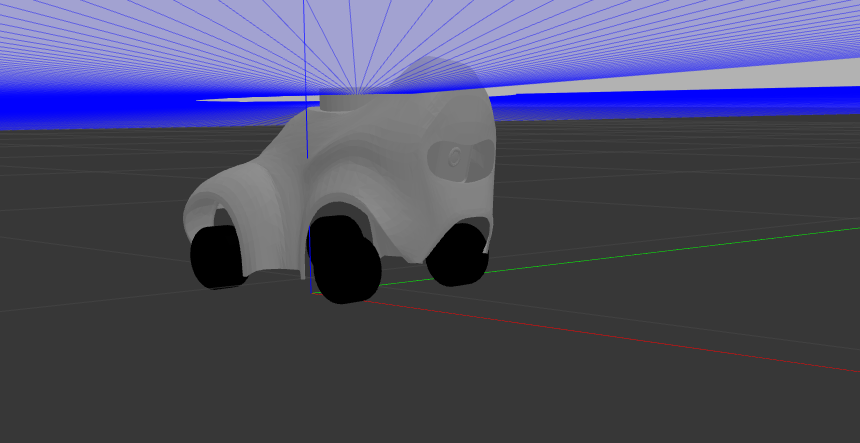
\includegraphics[height=3.2cm]{imagenes/etapa_deepracer_gazebo.png}\hfill
  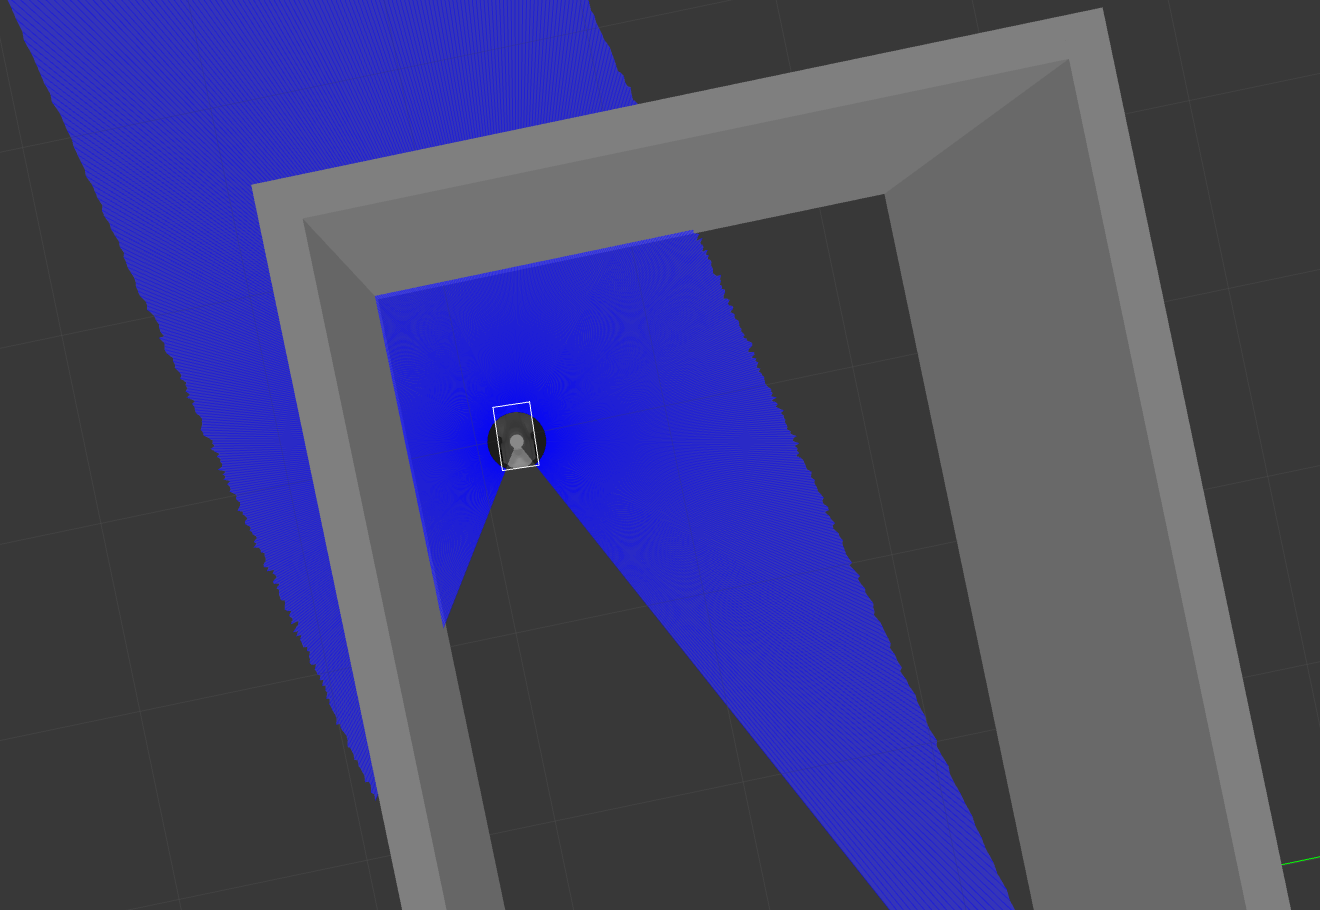
\includegraphics[height=3.2cm]{imagenes/etapa_pasillo_usta.png}
  \caption{Modelo propio del DonkeyCar en el visualizador de ROS~2 (izquierda) y modelo de AWS DeepRacer en ROS~2 Humble, en un mundo vacío (centro) y en el primer modelo del pasillo de la universidad (derecha).}
  \label{fig:etapas-plataforma}
\end{figure}

\subsection{Locomoción}
\label{sec:banda-muerta}
\label{sec:media-vuelta}

En simulación, el software de AWS, escrito para ROS~2 Foxy sobre Ubuntu 20.04, se migró a Humble sobre Ubuntu 22.04 con tres cambios en el sistema de control de articulaciones: la orden que activa los controladores pasó de \texttt{start} a \texttt{active}, y el componente que publica el estado de las articulaciones cambió de nombre y de tipo. En un mundo vacío (figura~\ref{fig:etapas-plataforma}, centro), el modelo funcionó con el láser y la cámara publicando a 62 cuadros por segundo, un factor de tiempo real de 1,00 y los siete controladores activos. El ángulo del volante se calcula con el modelo de bicicleta a partir de la orden de velocidad, con lo que el error de seguimiento de las trayectorias bajó a la mitad.

En los agentes físicos, cuya marcha se comprobó primero desde su interfaz web (anexo A, video 3), un puente traduce la orden de velocidad al variador y al servomotor. El agente no se mueve con velocidades pedidas por debajo de 0,40~m/s, de modo que se subió a ese valor la velocidad mínima de aproximación del controlador y el agente no tiene régimen de aproximación fina. Además, como la tracción funciona en lazo abierto, el puente tiene una escala por agente, ajustada en campo: 0,85 en el del piso 3 del edificio Catalayud y 0,9 en el del piso 4. Con la escala 1,0, el del piso 4 iba a 1,36~m/s y se pasaba de la meta; con 0,9 va a 0,74~m/s. Con la misma orden el motor retrocedía a 1,7 veces la velocidad de avance, por lo que la marcha atrás lleva una escala de 0,75.

La media vuelta es necesaria, puesto que cada misión empieza donde terminó la anterior y el siguiente usuario queda a menudo detrás del agente. En simulación la resuelve Nav2 con una inversión de marcha (anexo A, video 4), pero en el piso 4 de Catalayud, a la salida del pasillo de 2,5~m, abortó dos veces contra la pared, debido a que el planificador proponía cada segundo una maniobra distinta. Por esa razón se escribió una maniobra propia del agente, que alterna marcha atrás y avance con la dirección a tope, empieza hacia el costado con más espacio y corta cada tiempo cuando la huella prevista queda a menos de 0,10~m de un obstáculo. El coordinador la pide antes de una meta que queda a más de 110$^\circ$ del rumbo del agente y a más de 1,5~m, y si no se completa en 120~s, sigue Nav2. En la campaña con los agentes físicos se ejecutó 24 veces.

\subsection{Sensado}
\label{sec:odometria-laser}
\label{sec:imu}

El agente percibe con el láser, y como no tiene codificadores en las ruedas, su única odometría sale de comparar barridos sucesivos. En los pasillos rectos y uniformes del edificio Gregorio, donde cada barrido es casi igual al anterior, registró desde el 1,3~\% del avance real, en simulación, hasta el 73~\%, con un agente físico en el hall del piso 3. En los pisos 3 y 4 del edificio Catalayud, con la misma odometría y sin cambiar un parámetro, el error cayó por debajo del 5~\% (tabla~\ref{tab:odometria}).

El rumbo requirió la unidad inercial: con el láser solo, y con el agente quieto, derivó hasta 5,9$^\circ$ por minuto, y un giro de 90$^\circ$ hecho a mano se registró como 19,1$^\circ$. La Bosch BMI160 de la tarjeta, que el software del fabricante no usa, midió giros de 90$^\circ$ y 360$^\circ$ con un error de 0,1~\% a 1,3~\%. Se escribió un nodo que la lee y calibra el sesgo del giroscopio al arrancar, y un filtro de Kalman extendido toma de la odometría del láser el avance y de la unidad inercial el giro. En un giro de 90$^\circ$ contra una línea del piso, el filtro midió 90,17$^\circ$ en un agente y 88,38$^\circ$ en el otro, y con el agente quieto su rumbo se movió 0,3$^\circ$ o menos por minuto.

\subsection{Procesamiento y navegación autónoma}
\label{sec:primeros-entornos}
\label{sec:nav2-ackermann}

La navegación con mapa se adoptó después de evaluar un comportamiento reactivo. Un seguidor de paredes, probado en un tramo simulado del pasillo de la universidad de 7 por 3~m (figura~\ref{fig:etapas-plataforma}, derecha; anexo A, video 1), no se estabilizó con ninguna sintonía, dado que el radio de giro del agente deja muy poco margen en 3~m de ancho. En un pasillo ampliado de 15 por 5~m convergió por tramos, a 0,76~m de la pared frente a un objetivo de 0,5~m. En el modelo del piso 2 del edificio Gregorio, un pasillo de 44,25~m de largo y 5,09~m de ancho, se comprobaron los sensores y se construyó el primer mapa por localización y mapeo simultáneos (SLAM), que resultó de 23,04 por 15,72~m, la mitad del largo y el triple del ancho del pasillo.

Cada agente ejecuta su navegación a bordo, sobre Nav2. Su configuración por omisión supone tracción diferencial y propone trayectorias que un vehículo tipo automóvil no puede ejecutar. Por ello la pila se migró a Humble, la planificación global pasó al planificador híbrido A* de Smac con modelo Reeds-Shepp y el seguimiento al controlador Regulated Pure Pursuit, los dos con marcha atrás y con una velocidad deseada de 0,5~m/s. Del árbol de comportamiento se quitó la recuperación que gira sobre el propio eje. La cadena se puso en marcha con los siete pasos de la guía oficial \autocite{nav2setup}, de las transformaciones entre marcos de referencia al planificador y el controlador, y en el laboratorio quedó lista en 4~min 4~s en un agente y en 4~min 22~s en el otro. Los parámetros tienen una variante por distribución, y una prueba automática falla si se separan en algo distinto de las diferencias documentadas.

La banda muerta de tracción llevó a fijar la tolerancia de llegada con los agentes físicos en 0,5~m, mientras la simulación conserva 0,25~m, y la unidad inercial permitió reducir de 1,0 a 0,5~m el margen en el que Nav2 da la meta por alcanzada. La autonomía de las baterías limitó la duración de las sesiones de campo: las de los agentes se agotaron en dos sesiones, y durante la campaña el portátil se apagó dos veces.

\subsection{Comunicación}
\label{sec:dos-vehiculos}
\label{sec:red}

Como los agentes se mueven, el enlace tiene que ser inalámbrico. La red de la universidad quedó descartada, ya que aísla a sus clientes entre sí, no admite reservas de dirección y no se puede diagnosticar ni modificar. Tampoco servía una red móvil, pues el sistema está diseñado para funcionar sin salida a internet. Una red propia sobre Wi-Fi da control completo, direcciones fijas y posibilidad de medir, con el límite de que un enlace compartido no garantiza tiempos de entrega, por lo que el requisito de red fija cotas numéricas y se verifica midiendo.

Un enrutador, en el piso 4 del edificio Catalayud junto al punto de acceso de ese piso, reparte las direcciones de toda la red, y de él salen por cable los dos puntos de acceso: el del piso 4, en el mismo piso, y el del piso 3, con un cable que baja desde el piso 4 (figura~\ref{fig:red-topologia}). Los dos trabajan en modo puente, de manera que toda la instalación forma una sola subred, condición para que cada agente y el portátil se descubran. El enlace entre pisos va por cable, debido a que un repetidor usa la misma antena para enlazar y para sus clientes, con lo que pierde la mitad del caudal. En la banda de 2,4~GHz un barrido del sitio encontró 33 redes ajenas, de manera que se trabaja en la de 5~GHz, y el cambio de banda redujo el percentil 95 del tiempo de ida y vuelta de 20,76 a 11,12~ms. Hay un punto de acceso por piso, en canales que no se solapan, ya que la losa atenúa la señal. La tabla~\ref{tab:direcciones-red} da la dirección IP de cada equipo.

\begin{table}[H]
  \centering\footnotesize\setstretch{1.0}
  \caption{Direcciones IP de los equipos de la red en los pisos 3 y 4 del edificio Catalayud.}
  \label{tab:direcciones-red}
  \begin{tabular}{@{}>{\raggedright\arraybackslash}p{0.24\textwidth}>{\raggedright\arraybackslash}p{0.38\textwidth}>{\raggedright\arraybackslash}p{0.3\textwidth}@{}}
    \toprule
    \textbf{Equipo} & \textbf{Conexión} & \textbf{Dirección IP} \\ \midrule
    Enrutador TP-Link \mbox{TL-WR940N} & En el piso~4; cable a cada punto de acceso y red de respaldo a 2,4~GHz & \texttt{192.168.0.1/24}, fija \\ \addlinespace
    Punto de acceso del piso~3 & Cable entre pisos al enrutador; 5~GHz, canal~44 & --- \\ \addlinespace
    Punto de acceso del piso~4 & Cable al enrutador, en el mismo piso; 5~GHz, canal~36 & --- \\ \addlinespace
    Agente del piso~3 & Wi-Fi al punto de acceso de su piso & \texttt{192.168.0.102}, reservada en el enrutador \\ \addlinespace
    Agente del piso~4 & Wi-Fi al punto de acceso de su piso & \texttt{192.168.0.104}, reservada en el enrutador \\ \addlinespace
    Portátil & Wi-Fi a la red de respaldo del enrutador & \texttt{192.168.0.105}, asignada por el enrutador \\ \bottomrule
  \end{tabular}
\end{table}

Las fallas de la red no producían ningún mensaje de error y se encontraron al medir. Para trabajar en 5~GHz hubo que habilitar esa banda en los agentes. A sus tarjetas les faltaba la base de datos regulatoria del sistema operativo, que fija los canales en que puede emitir la radio, y sin ella las 31 frecuencias de 5~GHz quedaban en solo escucha: los agentes veían las redes, pero no podían transmitir en ellas. El defecto no produce ningún mensaje de error, de modo que el agente falla al conectarse sin informar de la causa, y se encontró al revisar el estado de cada frecuencia y no al contar las que la tarjeta lista. Se instaló esa base en los dos agentes, junto con un servicio que fija el dominio regulatorio en cada arranque, y al reiniciarlos cada tarjeta pasó de ninguno a 13 canales utilizables, entre ellos del 36 al 48 con 23~dBm, mientras el enlace pasó de 802.11n a 802.11ac. La otra falla fue un punto de acceso conectado a la vez por cable y por radio, que hacía que de 100 peticiones enviadas un agente recibiera 147.

En ROS~2 cada proceso se anuncia periódicamente a todos los demás, con lo que ese trabajo crece aproximadamente con el cuadrado del número de participantes. Con un agente su tarjeta trabajaba entre el 52~\% y el 63~\% de capacidad, mientras que al encender el segundo subió al 95~\% y Nav2 no alcanzó a arrancar. El coordinador y el grabador se llevaron por ello al portátil, que quedó como único interlocutor conocido de cada agente; los agentes no se ven entre sí, lo que coincide con el diseño, y el sistema completo volvió a entre el 68~\% y el 74~\% de la tarjeta.

\begin{figure}[H]
  \centering
  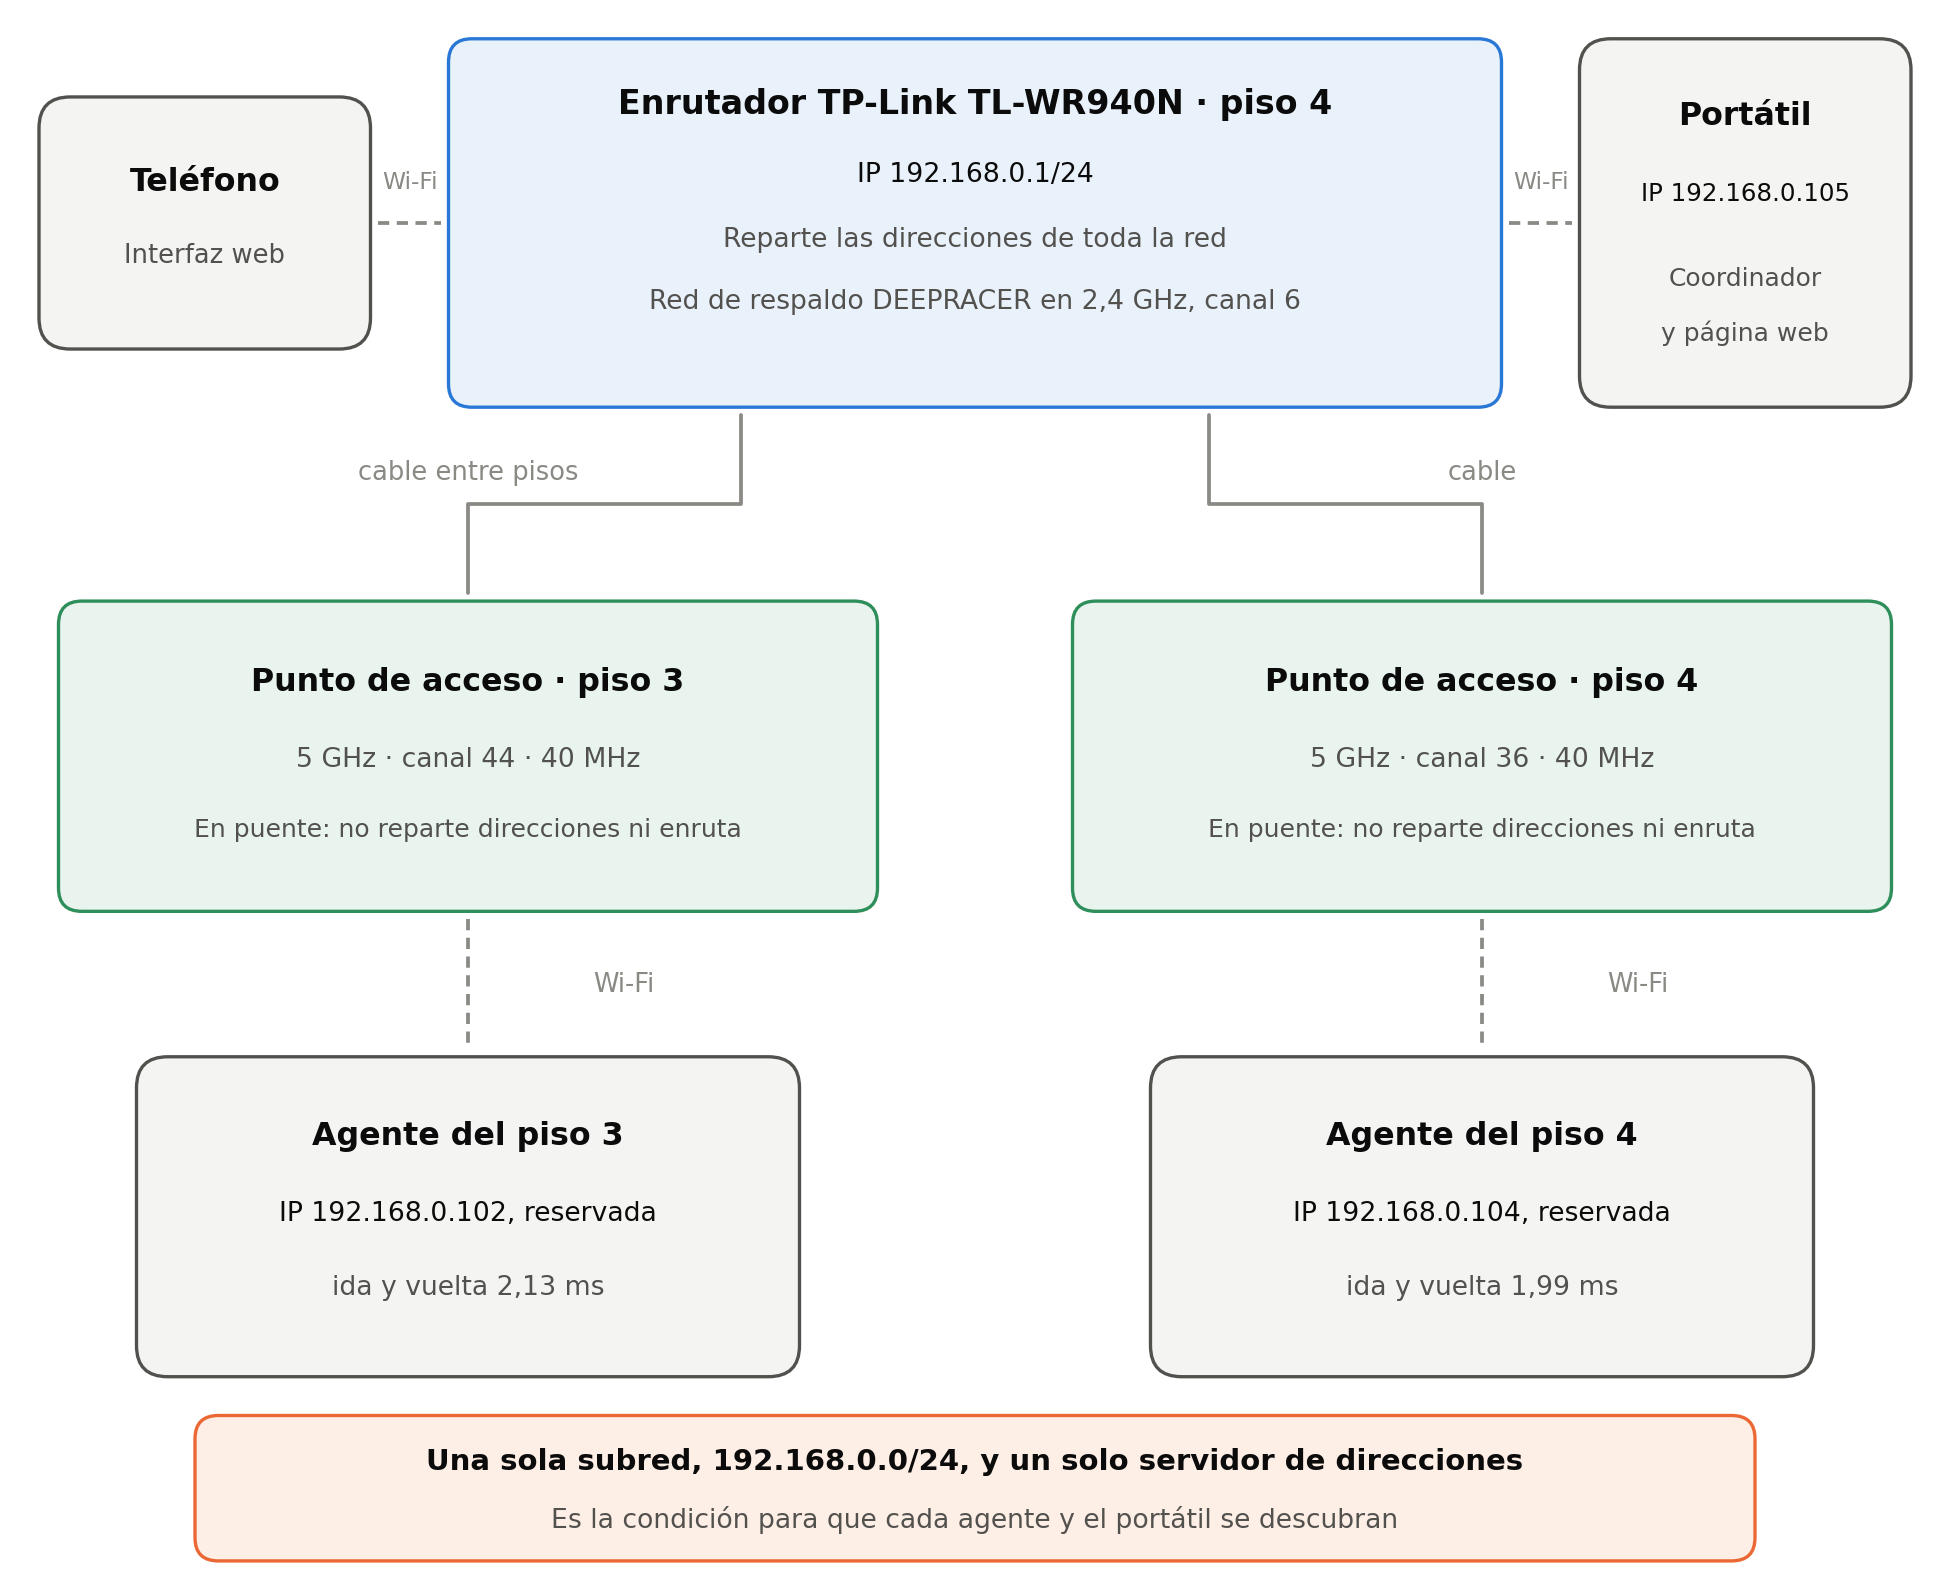
\includegraphics[width=0.9\textwidth]{imagenes/red_topologia.png}
  \caption{Montaje físico de la red en los pisos 3 y 4 del edificio Catalayud, con las direcciones IP de los equipos.}
  \label{fig:red-topologia}
\end{figure}

Las cotas del requisito, una mediana de 100~ms y un percentil 95 de 250~ms sin pérdidas, se fijaron antes de medir a partir del periodo de 0,5~s con que cada agente publica su estado, a 2~Hz. Con una latencia de ida de ese orden, la posición que recibe el coordinador llegaría atrasada una publicación, de modo que el límite es de 1~s de ida y vuelta, y las cotas dejan un margen de 10 veces en la mediana y de 4 en el percentil 95. Esa frecuencia alcanza para el uso que tiene el estado: el coordinador toma de él la posición de cada agente físico para decidir la media vuelta y para verificar la llegada, que comprueba con el agente ya detenido, mientras que el control del movimiento corre a bordo, en la navegación de cada agente. Entre los dos agentes, en la misma sala y sobre 600 mensajes, la mediana fue de 5,99~ms y el percentil 95 de 11,12~ms, sin pérdidas. En el montaje definitivo, con cada agente en el punto de acceso de su piso del edificio Catalayud, la ida y vuelta fue de 2,13 y 1,99~ms contra el enrutador, sin pérdidas ni duplicados, de modo que la red no limita el desempeño del sistema.

\subsection{Integración de los módulos}
\label{sec:integracion}
\label{sec:simulacion}
\label{sec:sim-a-vehiculos}

Los escenarios de los pisos 2 y 3 del edificio Gregorio se montaron en Gazebo~11 con ROS~2 Humble, cuyo enlace con el simulador aplica a todos los complementos el espacio de nombres del primer modelo cargado, lo que impidió tener dos agentes en un mismo proceso. Con los dos pisos en un mismo mundo, además, el láser simulado, de 10~m de alcance, veía paredes del otro piso en 61 de 1701 posiciones muestreadas. Por esas razones cada piso es un mundo distinto, con su propio proceso de simulación (figura~\ref{fig:sim-procesos}, izquierda), y los dos agentes comparten un dominio de comunicaciones, separados por espacio de nombres. Así integrado, el sistema completó una misión con relevo en 100,1~s. El mapa de navegación se calculó de la geometría del modelo, puesto que otro mapa construido con SLAM cubría el 35,5~\% del largo del pasillo, medía 15,0~m de ancho frente a los 5,3~m del mundo simulado, y el 74~\% de sus celdas ocupadas no tenía ninguna pared detrás.

Como los mundos simulados de los pisos 3 y 4 del edificio Catalayud salen del mismo levantamiento que sus mapas, el sistema también se comprobó en simulación en esos pisos (figura~\ref{fig:sim-procesos}, derecha), sin el protocolo de la campaña: de trece misiones, diez se completaron, tres se cancelaron a propósito y ninguna falló, con llegadas entre 0,067 y 0,206~m. La simulación sigue sin reproducir la odometría real, la respuesta de la tracción y la red entre pisos.

\begin{figure}[H]
  \centering
  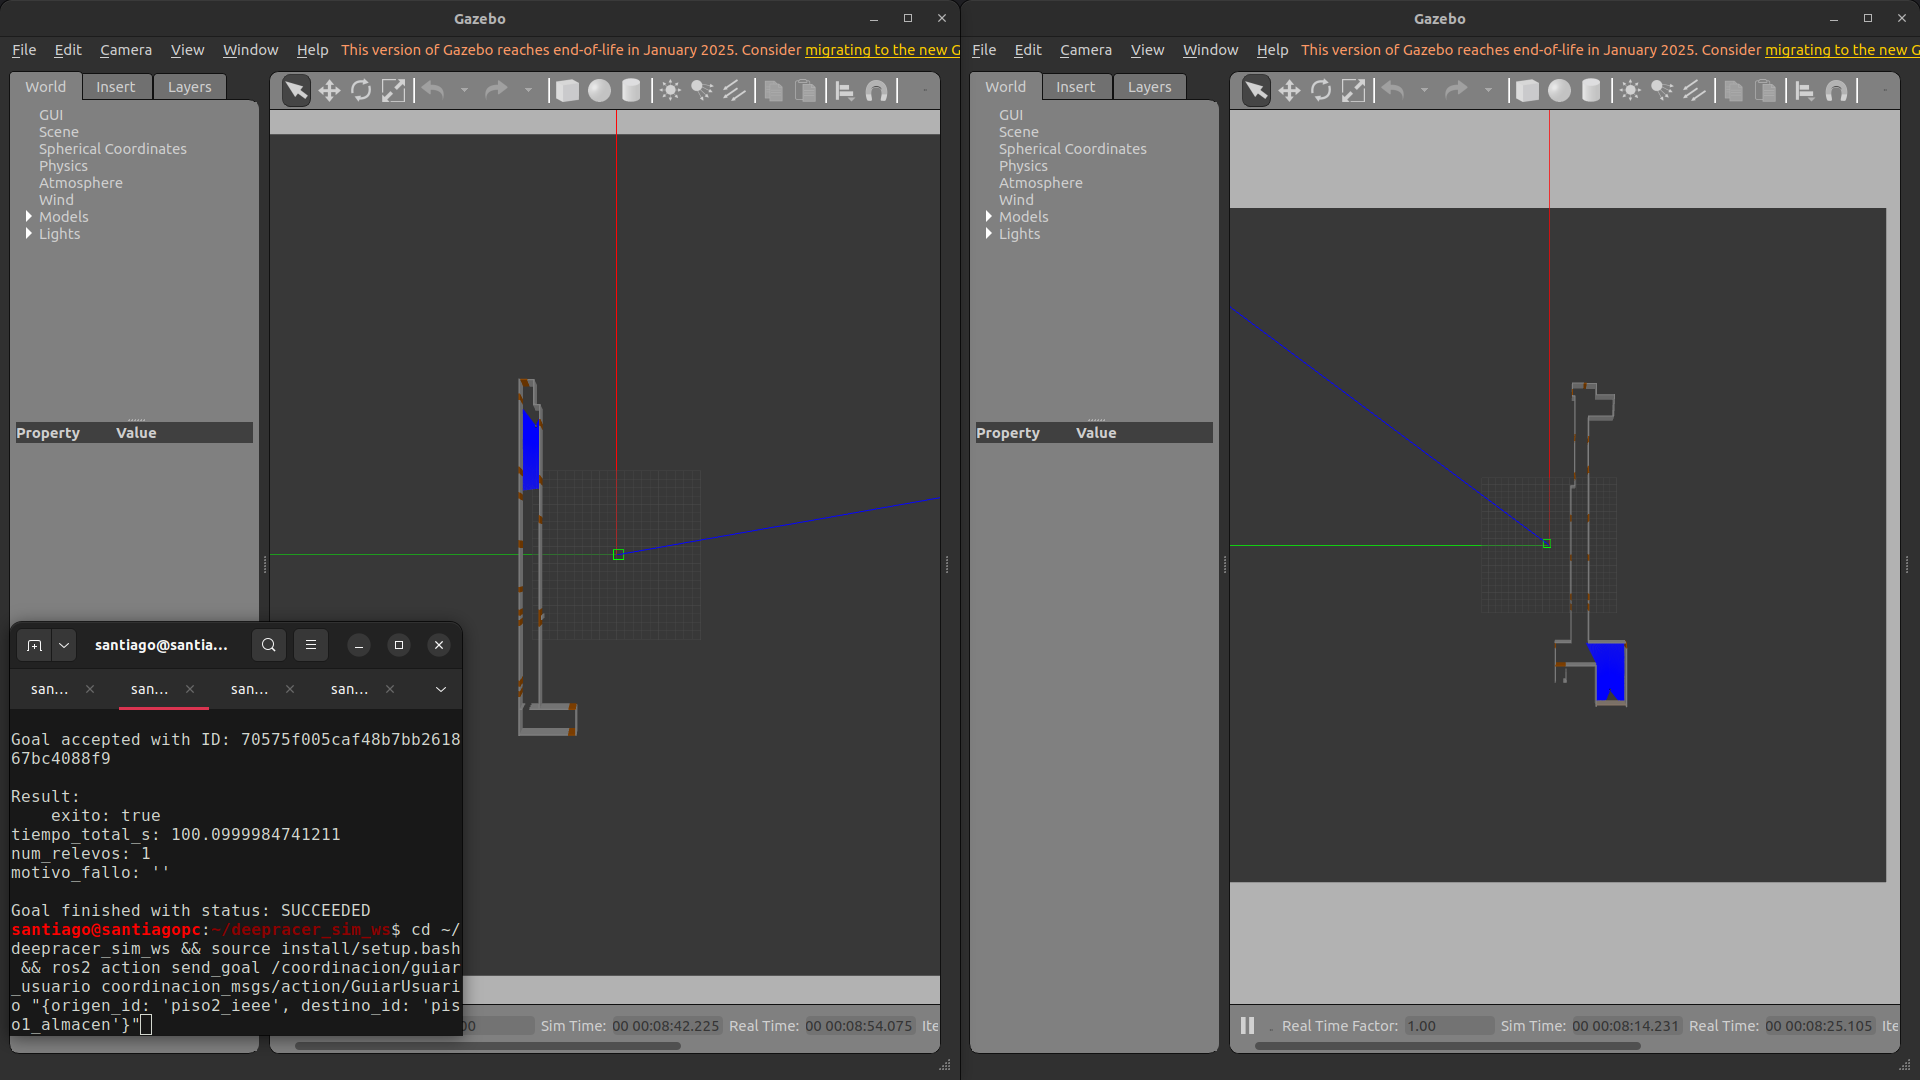
\includegraphics[height=4cm]{imagenes/simulacion_relevo_dos_procesos.png}\hfill
  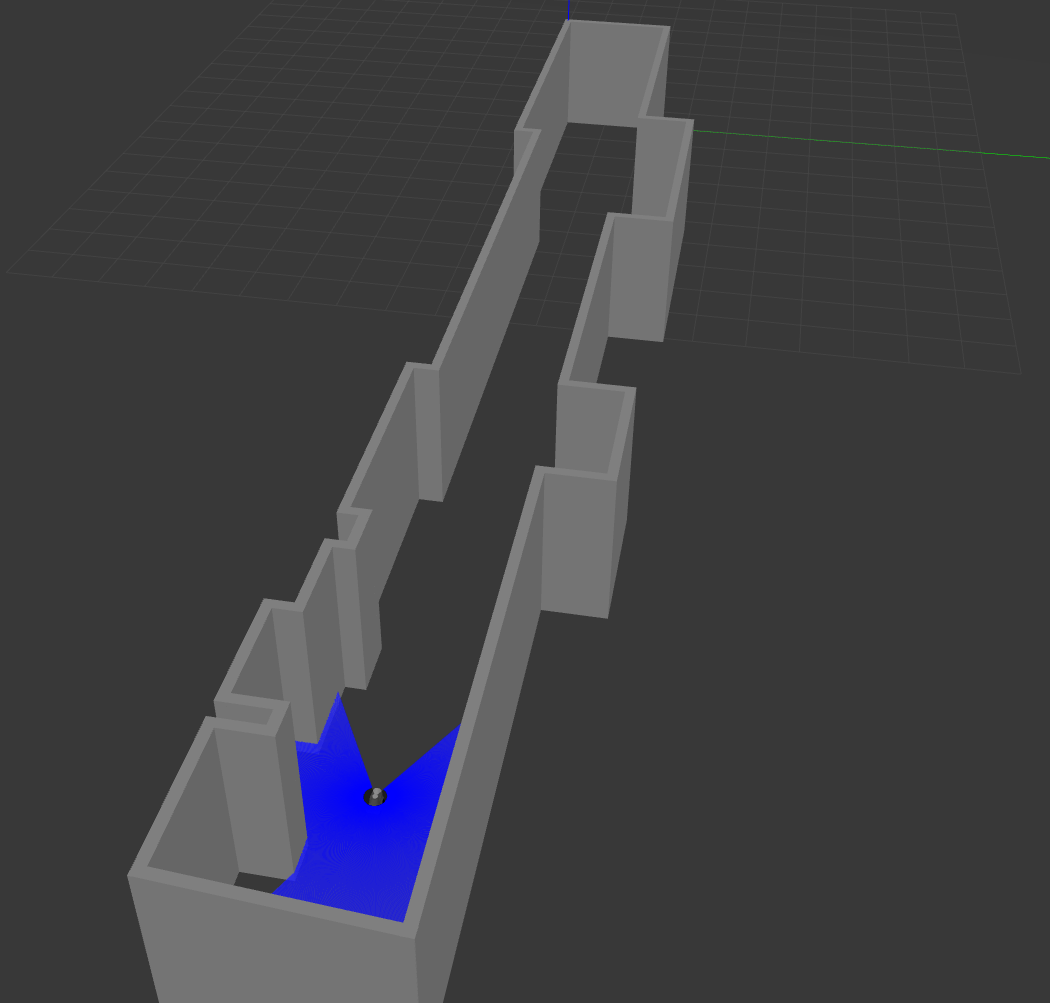
\includegraphics[height=4cm]{imagenes/simulacion_catalayud_piso3.png}\hfill
  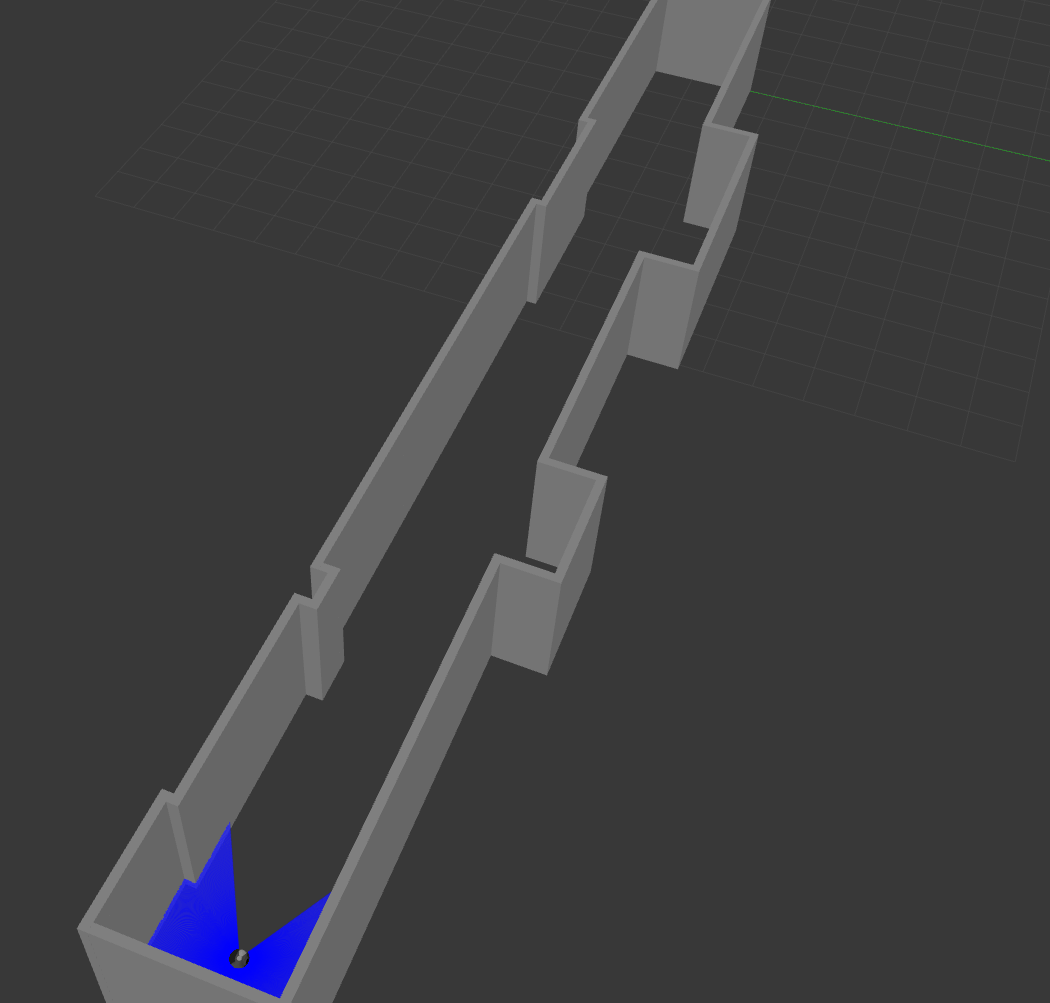
\includegraphics[height=4cm]{imagenes/simulacion_catalayud_piso4.png}
  \caption{Misión con relevo en simulación, con un proceso de Gazebo por piso (izquierda), y pisos 3 (centro) y 4 (derecha) del edificio Catalayud en simulación.}
  \label{fig:sim-procesos}
\end{figure}

Al llevar el sistema a los agentes físicos se mantuvo su estructura: un coordinador, un agente por piso, el relevo en la escalera y las reglas del contrato. También se mantuvo el código del coordinador, del planificador, de los mensajes y de la página, que compila sin cambios en las dos distribuciones de ROS~2. La integración con los agentes físicos se comprobó con seis pruebas de verificación sucesivas, cada una con un criterio escrito antes de ejecutarla (tabla~\ref{tab:pruebas-verificacion}).

\label{sec:pruebas-verificacion}
\begin{table}[H]
  \centering\footnotesize\setstretch{1.0}
  \caption{Pruebas de verificación de la demostración física, todas superadas al cerrar la toma de datos.}
  \label{tab:pruebas-verificacion}
  \begin{tabular}{@{}>{\raggedright\arraybackslash}p{0.3\textwidth}>{\raggedright\arraybackslash}p{0.64\textwidth}@{}}
    \toprule
    \textbf{Prueba} & \textbf{Criterio} \\ \midrule
    Actuación & El agente responde a las órdenes de dirección y tracción \\
    Odometría & Error de 10~\% o menos sobre un recorrido conocido de 5~m o más \\
    Navegación de un agente & Un agente llega de un punto a otro con Nav2, con la llegada verificada \\
    Dos agentes en la misma red & Los dos agentes y el coordinador coexisten sin conflicto de nombres \\
    Misión con relevo & Una misión con relevo sobre los dos agentes, con su registro \\
    Campaña con los agentes físicos & Entre 5 y 10 repeticiones del protocolo con su registro \\ \bottomrule
  \end{tabular}
\end{table}

Lo que cambió fue la implementación de los bloques (figura~\ref{fig:arquitectura-vehiculos} y tabla~\ref{tab:sim-vehiculos}).

\begin{figure}[H]
  \centering
  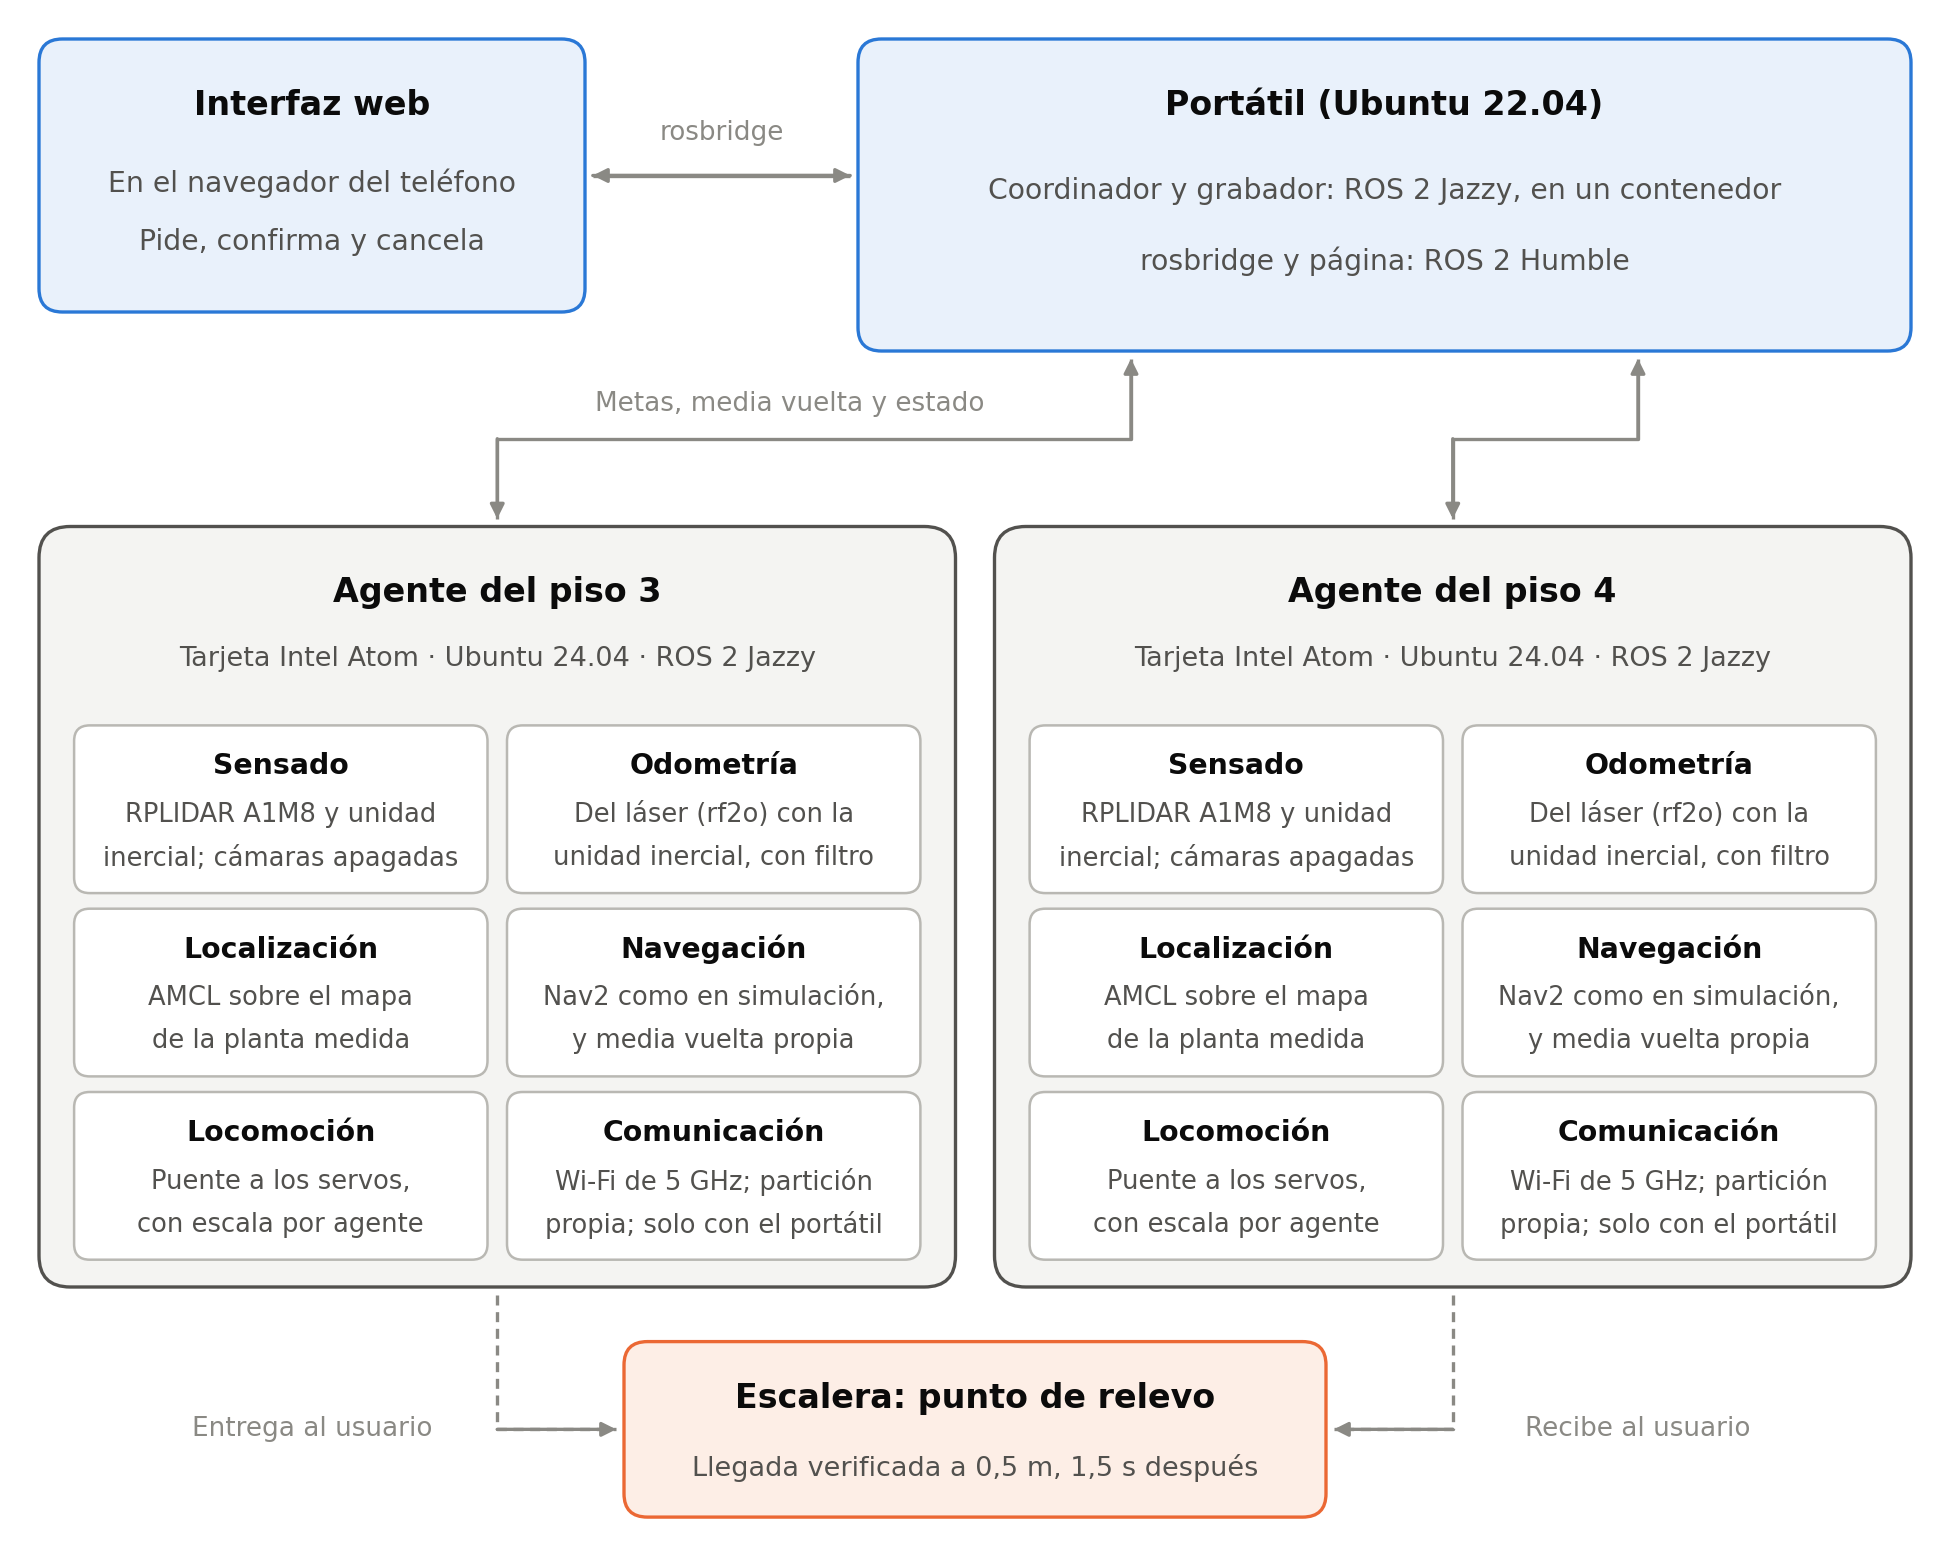
\includegraphics[width=0.82\textwidth]{imagenes/arquitectura_vehiculos.png}
  \caption{Arquitectura del sistema en la campaña con los agentes físicos.}
  \label{fig:arquitectura-vehiculos}
\end{figure}

\begin{table}[H]
  \centering\footnotesize\setstretch{1.0}
  \caption{Cambios en la implementación al pasar de la simulación a los agentes físicos.}
  \label{tab:sim-vehiculos}
  \begin{tabular}{@{}>{\raggedright\arraybackslash}p{0.13\textwidth}>{\raggedright\arraybackslash}p{0.205\textwidth}>{\raggedright\arraybackslash}p{0.285\textwidth}>{\raggedright\arraybackslash}p{0.30\textwidth}@{}}
    \toprule
    \textbf{Parte} & \textbf{En simulación} & \textbf{En los agentes físicos} & \textbf{Causa} \\ \midrule
    Distribución de ROS~2 & Humble en todos los componentes & Jazzy en los agentes y en el coordinador, en un contenedor del portátil; Humble en la página y en rosbridge & El software de la tarjeta solo existe para Jazzy y la simulación no existe en Jazzy \\ \addlinespace
    Coordinador & En el portátil, junto a los dos simuladores & En el portátil, después de un intento en uno de los agentes & En una tarjeta, con las dos navegaciones encendidas, la carga subió de 6 a entre 17 y 33 y Nav2 no arrancaba \\ \addlinespace
    Comunicación & Un computador; un espacio de nombres por agente & Red inalámbrica; una partición por agente y topología en estrella hacia el portátil & Los tópicos del fabricante no llevan espacio de nombres, y el descubrimiento saturaba las tarjetas \\ \addlinespace
    Locomoción & Complemento Ackermann de Gazebo & Puente de la orden de velocidad a los servos, con una escala por agente & La tracción real tiene banda muerta y funciona en lazo abierto \\ \addlinespace
    Sensado & Láser simulado de 10~m de alcance & RPLIDAR A1M8 y la unidad inercial de la tarjeta; cámaras apagadas & Las cámaras no se usan y cargaban la tarjeta \\ \addlinespace
    Odometría & La del simulador & La del láser, combinada con la unidad inercial & El agente no tiene codificadores en las ruedas \\ \addlinespace
    Mapa & Calculado del mundo simulado & Derivado de la planta medida con flexómetro & El mapeo con SLAM a bordo no entregó un mapa utilizable \\ \addlinespace
    Escenario & Pisos 2 y 3 del edificio Gregorio & Pisos 3 y 4 del edificio Catalayud, levantados con flexómetro & Tránsito de personas, mundo simulado mal medido y pasillos uniformes en Gregorio \\ \addlinespace
    Llegada & Tolerancia de 0,25~m & Tolerancia de 0,5~m, verificada con la pose del agente 1,5~s después de que Nav2 da la meta por alcanzada & Banda muerta; el agente sigue rodando cuando Nav2 declara la llegada \\ \addlinespace
    Media vuelta & La planifica Nav2 & Maniobra propia del agente, vigilada con el láser y el mapa & La de Nav2 abortó contra la pared en el piso 4 de Catalayud \\ \bottomrule
  \end{tabular}
\end{table}

% =====================================================================
\section{Tercer objetivo específico: interfaz móvil}
\label{sec:oe3}
\label{sec:ajustes-campo}

El objetivo pide una interfaz móvil basada en la selección de localizaciones de origen y destino, y se cumplió con una página web que se abre en el navegador del teléfono, porque un usuario ocasional no va a instalar nada para preguntar por un salón. La página funciona sin salida a internet, sin bibliotecas ni recursos externos: son un archivo HTML, una hoja de estilo y dos programas en JavaScript, que sirve el propio portátil en el puerto 8000. Se comunica con ROS~2 por el puente \textit{rosbridge}, en el puerto 9090, que no tiene autenticación, así que el firewall del portátil solo admite conexiones a esos dos puertos desde la red de los agentes.

\subsection{Selección de origen y destino}

El usuario elige el origen en una lista y el destino en un catálogo con búsqueda por nombre, donde cada destino muestra su piso y, si queda en el otro piso, la marca «con relevo» (figura~\ref{fig:hri}, izquierda). Los dos ascensores del edificio Catalayud se llamaban igual en la lista, y en una misión se eligió el del piso equivocado, así que los nombres repetidos se muestran con su piso, como «Ascensor (piso 3)». Durante la misión, la página muestra el texto que redacta el coordinador, el agente que está guiando, hacia dónde va y la distancia restante, y una franja de cinco pasos marca el paso actual (figura~\ref{fig:hri}, centro).

\begin{figure}[H]
  \centering
  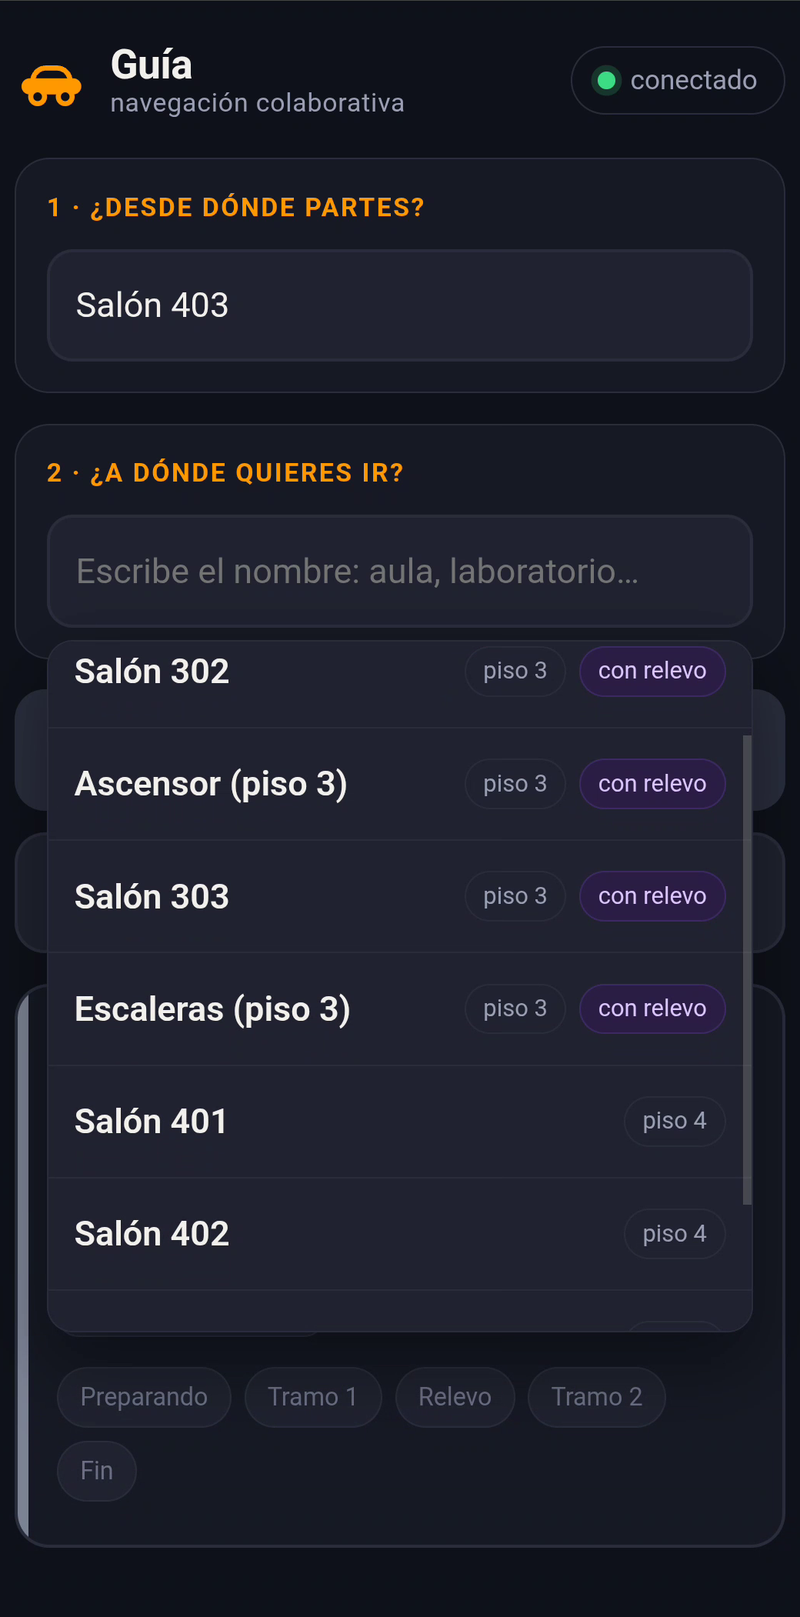
\includegraphics[height=9.2cm]{imagenes/hri_catalogo.png}\hspace{0.8cm}
  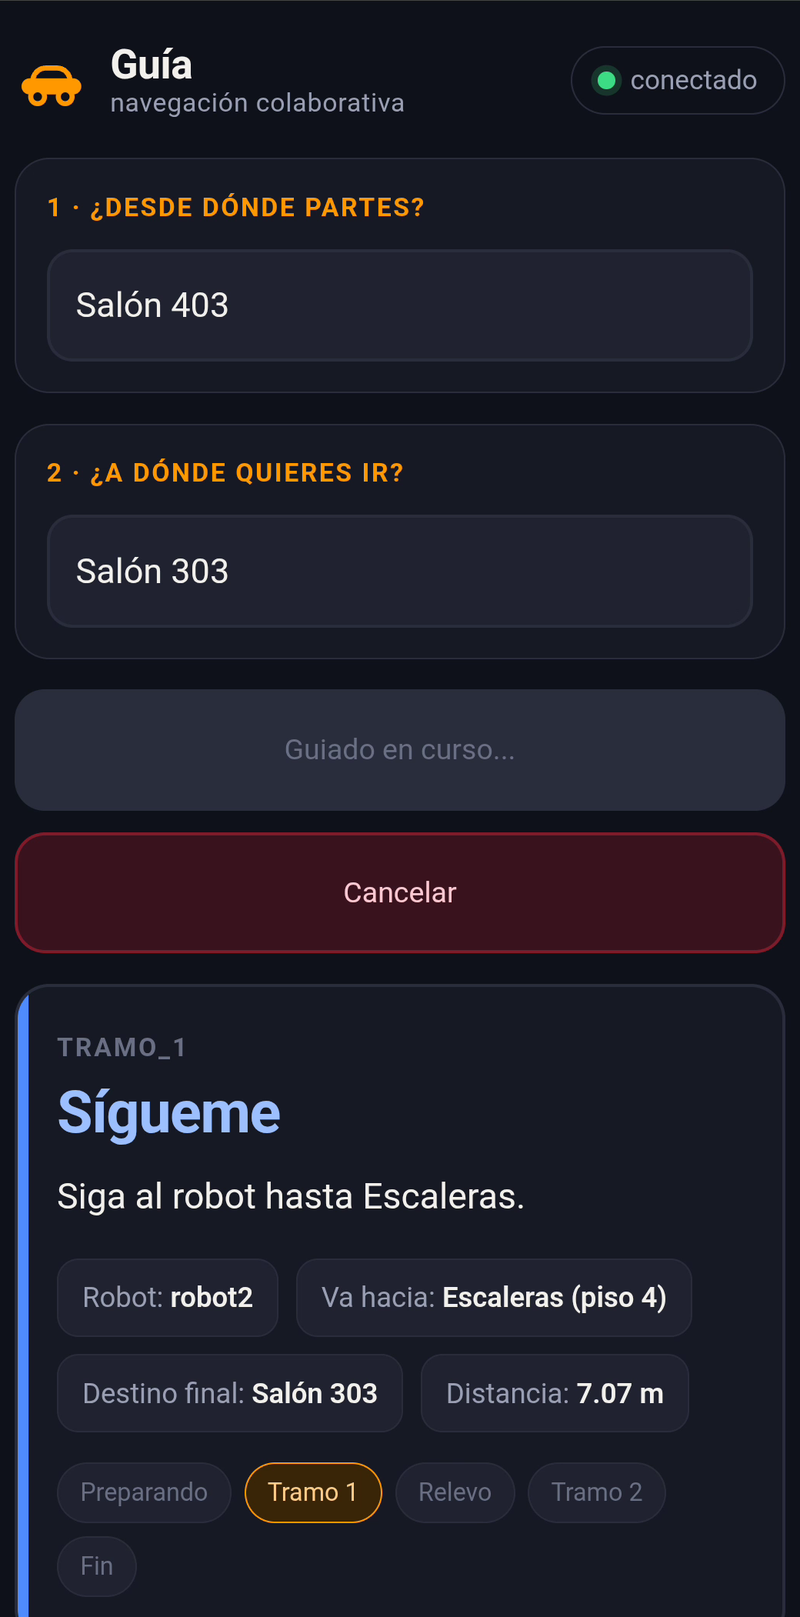
\includegraphics[height=9.2cm]{imagenes/hri_seguimiento.png}\hspace{0.8cm}
  \begin{minipage}[b]{4.05cm}
    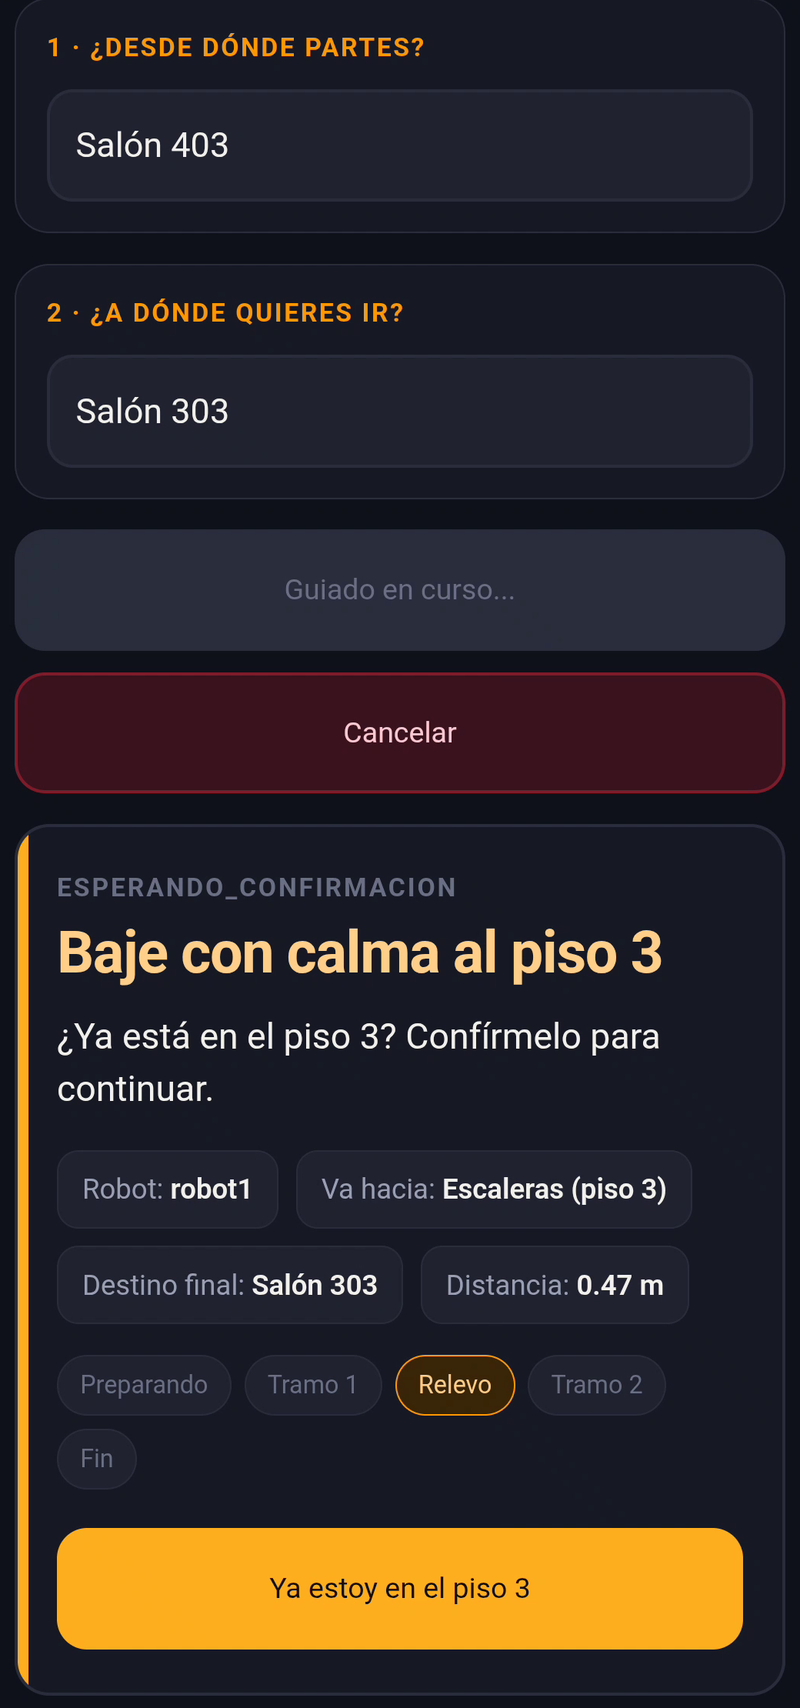
\includegraphics[trim=0 0 0 818,clip,width=\linewidth]{imagenes/hri_confirmacion_piso.png}\\[0.2cm]
    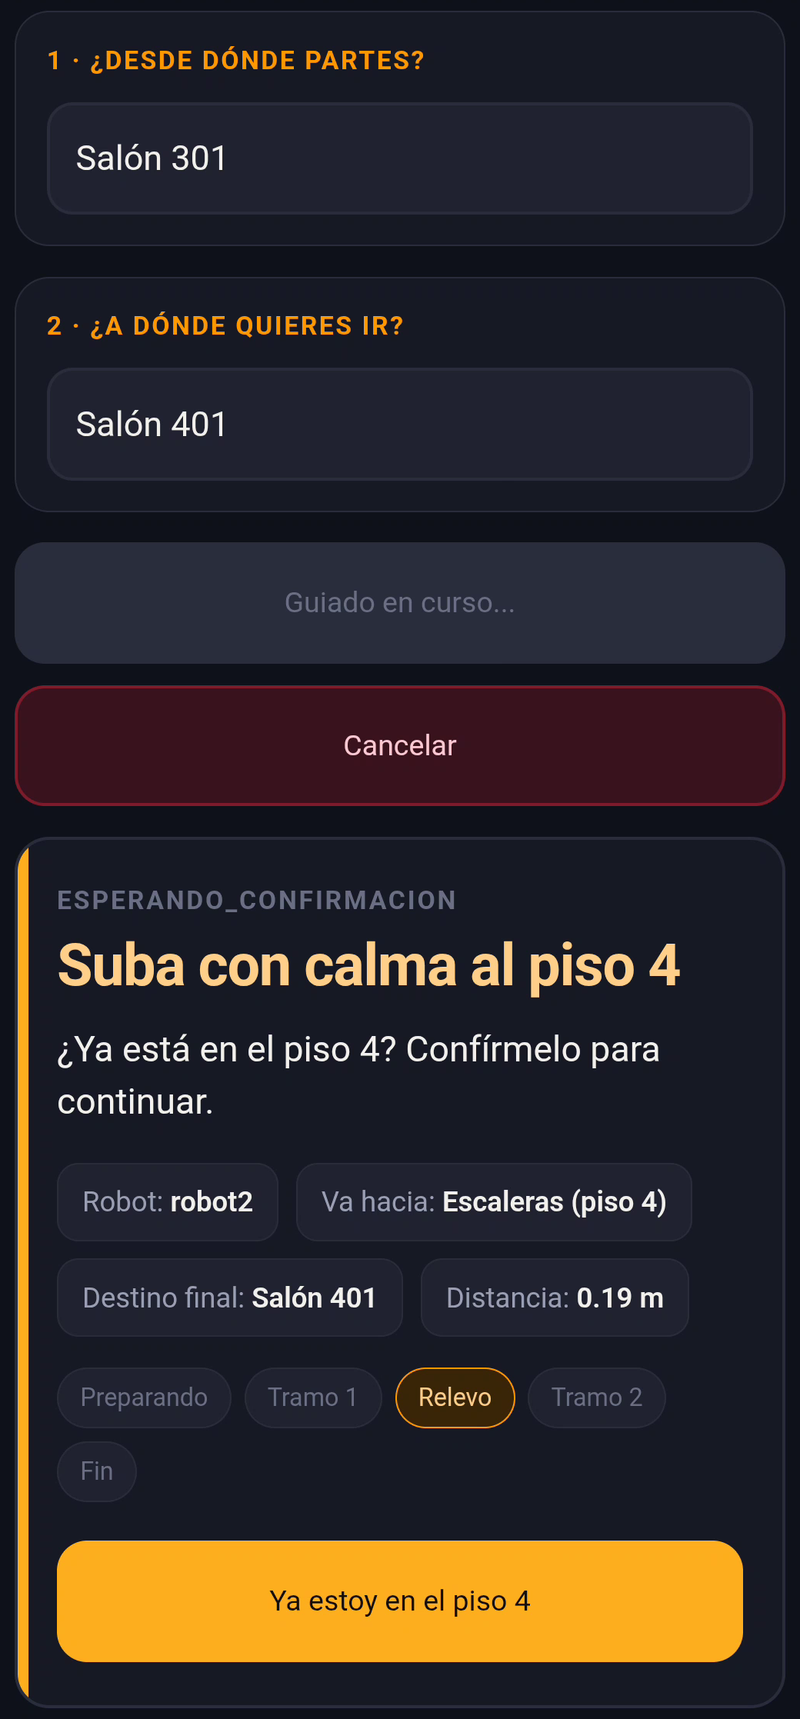
\includegraphics[trim=0 0 0 832,clip,width=\linewidth]{imagenes/hri_confirmacion_subida.png}
  \end{minipage}
  \caption{Interfaz web en el teléfono durante las pruebas con los agentes físicos (anexo A, video 8): catálogo de destinos (izquierda), primer tramo de una misión (centro) y espera de confirmación al bajar y al subir (derecha).}
  \label{fig:hri}
\end{figure}

\subsection{Confirmación de cambio de piso}

En una misión entre pisos, el segundo agente llega a su escalera y no puede saber si el usuario ya cambió de piso. Por esa razón, cuando llega a su punto de transferencia, el coordinador pasa a la etapa de espera y la página muestra un botón para confirmar el cambio de piso (figura~\ref{fig:hri}, derecha), con un texto que depende del sentido, como «Suba con calma al piso 4» o «Baje con calma al piso 3». A los 60~s sin confirmación aparece un aviso, y a los 120~s la misión termina como fallida. Los plazos se cuentan desde que llega el agente, y si el usuario confirma antes, la confirmación se retiene y se aplica al llegar.

\subsection{Cancelación}

La cancelación requirió registrar en el servidor de acción la función que la responde, ya que ROS~2 rechaza por omisión toda cancelación sin esa función. Al cancelar, la misión pasa por la etapa de cancelación, el agente activo regresa al punto de transferencia de su piso y la misión cierra como fallida con un texto que lo dice. Con los agentes físicos se cancelaron seis misiones en los pisos 3 y 4 del edificio Catalayud, al menos una en cada etapa (anexo A, video 8), y en las seis el agente volvió a su escalera, a entre 0,07 y 0,34~m de su punto. La interfaz se verificó contra el coordinador real y en un teléfono conectado a la red de los agentes, donde se operó una misión completa con relevo sin tocar el computador.

% =====================================================================
\section{Cuarto objetivo específico: evaluación experimental}
\label{sec:protocolo}

La evaluación se hizo con las cuatro métricas que nombra el objetivo: tiempo de respuesta, tiempo de asignación, tasa de éxito y continuidad del servicio entre niveles.

\subsection{Métricas y criterio de éxito}

El protocolo se escribió antes de instrumentar el sistema, porque un protocolo redactado después de ver los datos tiende a acomodarse a lo que salió. Fija las métricas con su definición operativa (tabla~\ref{tab:metricas}), el criterio de éxito, el tamaño de muestra y una lista cerrada de causas de descarte.

\begin{table}[H]
  \centering\footnotesize\setstretch{1.0}
  \caption{Definición operativa de las cuatro métricas del anteproyecto.}
  \label{tab:metricas}
  \begin{tabular}{@{}>{\raggedright\arraybackslash}p{0.2\textwidth}>{\raggedright\arraybackslash}p{0.36\textwidth}>{\raggedright\arraybackslash}p{0.36\textwidth}@{}}
    \toprule
    \textbf{Métrica} & \textbf{Inicio} & \textbf{Fin} \\ \midrule
    Tiempo de respuesta & El coordinador acepta la solicitud & Primera de tres muestras seguidas de la odometría del agente asignado con velocidad de al menos 0,02~m/s \\ \addlinespace
    Tiempo de asignación & Primera publicación de la etapa recibida & Primera publicación del primer tramo, con el agente asignado \\ \addlinespace
    Tasa de éxito & \multicolumn{2}{p{0.72\textwidth}}{Proporción de misiones exitosas sobre las ejecuciones válidas} \\ \addlinespace
    Continuidad entre niveles & El primer agente alcanza su punto de transferencia & Primer movimiento del segundo agente \\ \bottomrule
  \end{tabular}
\end{table}

Una misión es exitosa si la pose final del agente, en su odometría, está a 0,25~m o menos del destino declarado en el catálogo (0,5~m en los agentes físicos), si llegó a la etapa completada sin pasar por fallida y, cuando era entre pisos, si hubo un relevo. El éxito se mide contra la odometría del agente, sin tomar por válido el resultado que devuelve Nav2: en las primeras pruebas en simulación, una de tres metas devolvió éxito con el agente a 0,296~m.

\subsection{Campañas de evaluación}

La campaña en simulación, en los pisos 2 y 3 del edificio Gregorio (anexo A, video 6), tiene treinta misiones en dos grupos de quince: en las de un mismo piso no hay relevo y sirven de comparación, y en las de dos pisos hay un relevo. Los pares de origen y destino salen de un sorteo cuya semilla es la fecha en que se hace, entre los puntos del catálogo menos los dos puntos de transferencia, que dan 392 pares posibles dentro de un mismo piso y 420 entre pisos, y el listado se guarda en el repositorio antes de la primera ejecución. Las diez primeras misiones, con la semilla 20260822, dejaban el grupo con relevo como el único que navegaba por el piso 3 de Gregorio, por lo que las veinte restantes se sortearon de nuevo con la semilla 20260904, para que cada grupo quedara repartido entre los dos pisos.

Una ejecución fallida cuenta como fallo y solo se descarta si la causa es ajena al sistema y está en la lista cerrada. Esa lista admite la caída del simulador, un controlador del agente que no se activa, el factor de tiempo real por debajo de 0,99, un fallo de la máquina anfitriona o una cancelación por una causa externa anotada antes de conocer el resultado. Si los descartes superan el 20~\%, la campaña no es válida. Para que las métricas temporales valgan, la simulación debe ejecutarse a tiempo real, y en las treinta misiones el factor de tiempo real tuvo un mínimo de 0,9917 y una media de 0,9973.

La campaña con los agentes físicos en los pisos 3 y 4 del edificio Catalayud (anexo A, video 7) parte de diez misiones sorteadas con la semilla 20261013, cinco de subida y cinco de bajada. Se ejecutaron en ese orden y sin reubicar los agentes entre misiones, como ocurriría en la operación real.

\subsection{Instrumentación y análisis}
\label{sec:instrumentacion}

Cada misión deja una grabación de datos de ROS (\textit{rosbag}) con los tópicos del coordinador y de los dos agentes. A partir de ella, un programa compone el registro de la misión (figura~\ref{fig:instrumentacion}, abajo), en un formato validado contra un esquema, y otro comprueba la integridad de los registros y calcula las cuatro métricas con sus intervalos de confianza. Con los agentes físicos, la llegada la verifica el coordinador con la pose que publica el agente, 1,5~s después de que Nav2 la da por alcanzada (figura~\ref{fig:instrumentacion}, arriba). En las llegadas medidas en el piso 4 del edificio Catalayud, el agente estaba a entre 0,53 y 0,62~m de la meta en la última orden de avance, y un segundo después, ya quieto, a entre 0,09 y 0,53~m.

\begin{figure}[H]
  \centering
  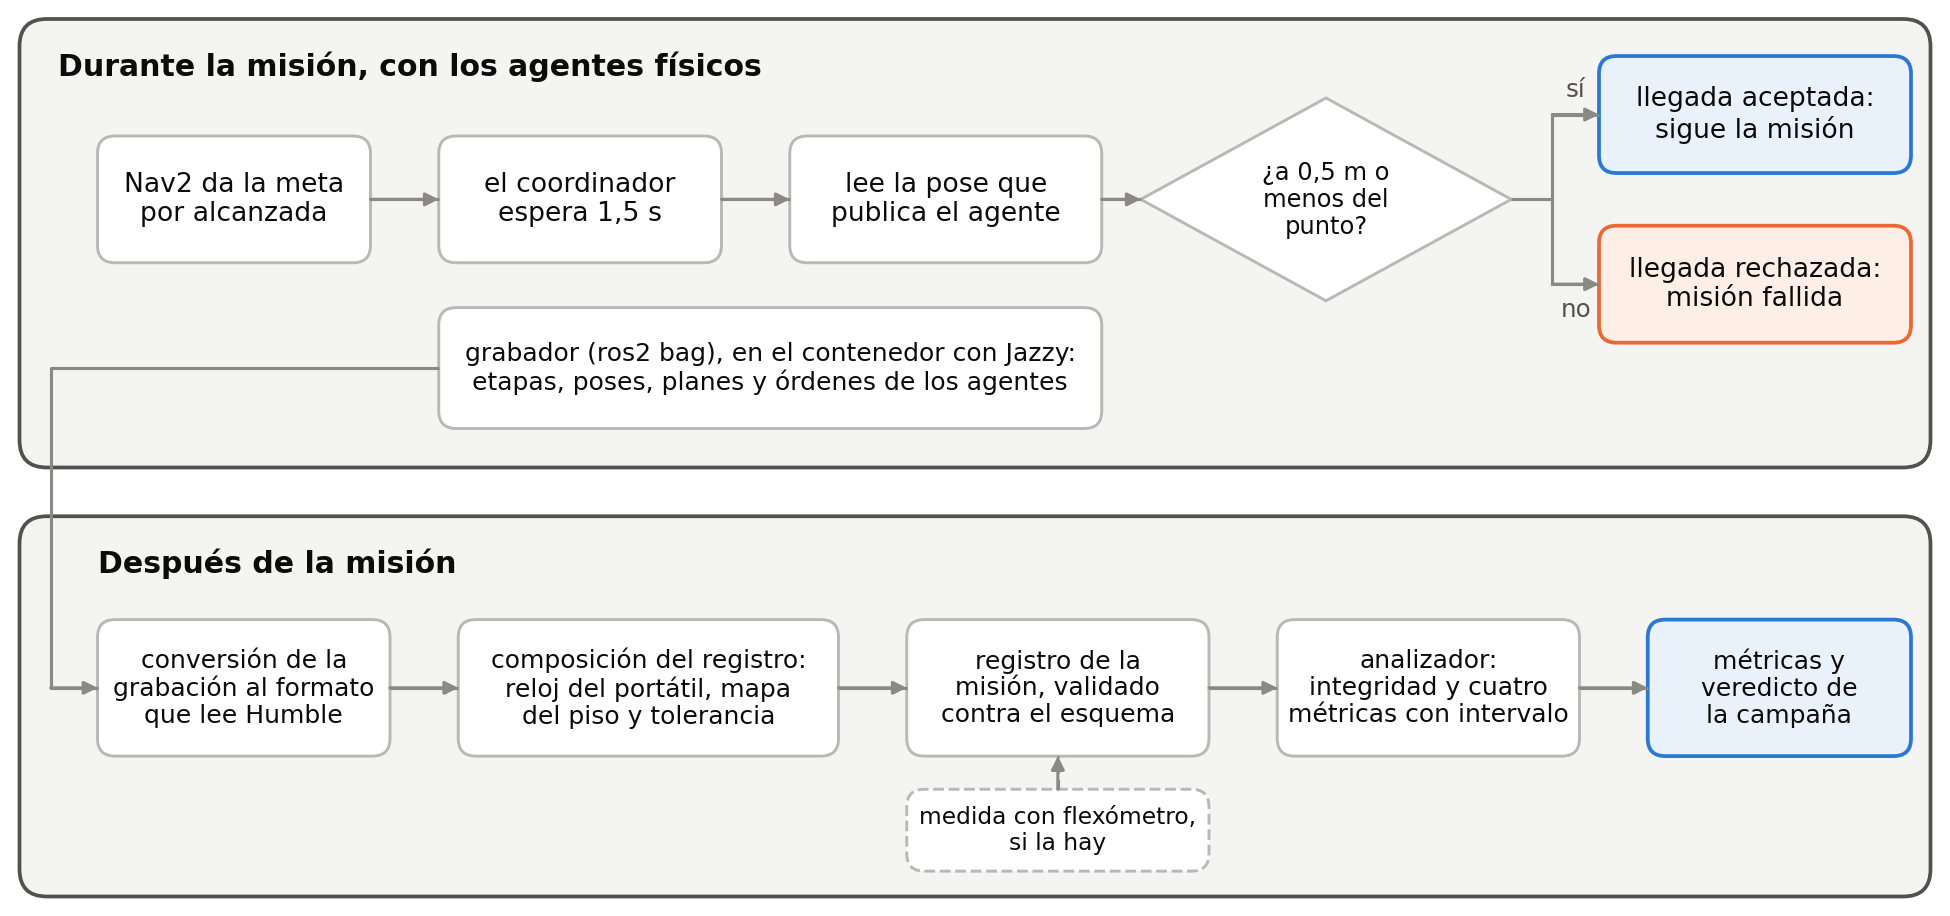
\includegraphics[width=\textwidth]{imagenes/instrumentacion.png}
  \caption{Instrumentación de una misión: verificación de la llegada con los agentes físicos (arriba) y camino de la grabación hasta las métricas (abajo).}
  \label{fig:instrumentacion}
\end{figure}

% =====================================================================
\section{Cumplimiento de los objetivos específicos}
\label{sec:cumplimiento}

Un objetivo se considera cumplido cuando todos sus requisitos tienen verificada la prueba que los declara cumplidos (tabla~\ref{tab:cumplimiento}). Las siete restricciones del alcance también quedaron verificadas, con lo que la matriz cierra con treinta y seis de treinta y seis.

\begin{table}[H]
  \centering\footnotesize\setstretch{1.0}
  \caption{Cumplimiento de cada objetivo específico: cómo se cumplió, requisitos verificados y evidencia.}
  \label{tab:cumplimiento}
  \begin{tabular}{@{}>{\raggedright\arraybackslash}p{0.15\textwidth}>{\raggedright\arraybackslash}p{0.41\textwidth}>{\raggedright\arraybackslash}p{0.1\textwidth}>{\raggedright\arraybackslash}p{0.26\textwidth}@{}}
    \toprule
    \textbf{Objetivo} & \textbf{Cómo se cumplió} & \textbf{Requisitos} & \textbf{Evidencia} \\ \midrule
    1. Arquitectura funcional & Matriz de requisitos, escenarios en los edificios Gregorio y Catalayud, asignación por piso con un planificador comprobado en 930 combinaciones y contrato de interfaces & 10 de 10 & Relevo en simulación y con los agentes físicos (anexo A, videos 5 a 7) \\ \addlinespace
    2. Plataforma robótica & Dos agentes sobre AWS DeepRacer con locomoción, sensado, procesamiento y comunicación integrados & 6 de 6 & Seis pruebas de verificación superadas (anexo A, videos 3, 4 y 7) \\ \addlinespace
    3. Interfaz móvil & Página web con selección de origen y destino, confirmación de cambio de piso y cancelación & 6 de 6 & Probada en un teléfono con los agentes físicos (anexo A, video 8) \\ \addlinespace
    4. Evaluación & Cuatro métricas con definición operativa, treinta misiones en simulación y nueve con los agentes físicos & 7 de 7 & Registros de cada misión (anexo B) y campañas (anexo A, videos 6 y 7) \\ \bottomrule
  \end{tabular}
\end{table}
